\documentclass[11pt,a4paper]{report}

% ============================================================
% Metadonnees du rapport -- a completer si necessaire
% ============================================================
\newcommand{\reportTitle}{VisionInspectIA}
\newcommand{\reportSubtitle}{AI-Powered Visual Inspection Platform for Bottle Defect Detection}
\newcommand{\reportKind}{Rapport de stage --- Programme AI/ML Internship}

\newcommand{\stagiaireNom}{Aymen Chiab}
\newcommand{\organisme}{TechSkillHub (programme \`a distance, www.techskillhub.tech)}
\newcommand{\identifiantStagiaire}{TSH/A5E51B1E}
\newcommand{\domaineStage}{AI / ML}
\newcommand{\dureeStage}{1 mois (4 semaines), \`a partir du 04 ao\^ut 2026}
\newcommand{\encadrant}{[\`A COMPL\'ETER]}
\newcommand{\etablissement}{[\`A COMPL\'ETER]}
\newcommand{\anneeUniv}{[\`A COMPL\'ETER]}
\newcommand{\dateFin}{[\`A COMPL\'ETER]}

% ============================================================
% Preambule -- VisionInspectIA, rapport de stage
% ============================================================
\usepackage[utf8]{inputenc}
\usepackage[T1]{fontenc}
\usepackage[french]{babel}
\usepackage[a4paper,margin=2.5cm,headheight=14pt]{geometry}

\usepackage{xcolor}
\usepackage{graphicx}
\usepackage{float}
\usepackage{booktabs}
\usepackage{longtable}
\usepackage{tabularx}
\usepackage{array}
\usepackage{amsmath}
\usepackage{amssymb}
\usepackage{enumitem}
\usepackage{listings}
\usepackage{fancyhdr}
\usepackage{tikz}
\usetikzlibrary{arrows.meta,positioning,shapes.geometric,shadows}
\usepackage{caption}
\usepackage{subcaption}
\usepackage{titlesec}
\usepackage{setspace}
\usepackage{csquotes}

% hyperref en dernier
\usepackage[colorlinks=true,linkcolor=accentdark,citecolor=accentdark,urlcolor=accent,pdfborder={0 0 0}]{hyperref}
% cleveref a pose un probleme de compatibilite avec cette distribution ;
% on retombe sur \ref simple, plus robuste, plutot que de bloquer la compilation.
\providecommand{\Cref}[1]{\ref{#1}}
\providecommand{\cref}[1]{\ref{#1}}

% ----------------------------------------------------------------
% Palette (bleu fonce / bleu / gris / blanc)
% ----------------------------------------------------------------
\definecolor{accentdark}{HTML}{1F3B57}
\definecolor{accent}{HTML}{2E5A88}
\definecolor{accentlight}{HTML}{DCE6F0}
\definecolor{graybg}{HTML}{F2F2F2}
\definecolor{graytext}{HTML}{555555}

% ----------------------------------------------------------------
% Titres de chapitres/sections
% ----------------------------------------------------------------
\titleformat{\chapter}[display]
  {\normalfont\bfseries\color{accentdark}}
  {\Large\MakeUppercase{\chaptertitlename}~\thechapter}
  {8pt}{\Huge}
\titleformat{\section}
  {\normalfont\Large\bfseries\color{accent}}{\thesection}{0.6em}{}
\titleformat{\subsection}
  {\normalfont\large\bfseries\color{accentdark}}{\thesubsection}{0.6em}{}

% ----------------------------------------------------------------
% En-tetes / pieds de page
% ----------------------------------------------------------------
\pagestyle{fancy}
\fancyhf{}
\renewcommand{\headrulewidth}{0.4pt}
\renewcommand{\footrulewidth}{0.2pt}
\fancyhead[L]{\small\textcolor{graytext}{VisionInspectIA --- Rapport de stage}}
\fancyhead[R]{\small\textcolor{graytext}{\leftmark}}
\fancyfoot[C]{\small\thepage}

% ----------------------------------------------------------------
% Listings (extraits de code)
% ----------------------------------------------------------------
\lstset{
  basicstyle=\ttfamily\small,
  breaklines=true,
  frame=single,
  rulecolor=\color{graytext},
  backgroundcolor=\color{graybg},
  numbers=left,
  numberstyle=\tiny\color{graytext},
  keywordstyle=\color{accentdark}\bfseries,
  commentstyle=\color{graytext}\itshape,
  stringstyle=\color{accent},
  showstringspaces=false,
  tabsize=2,
}

% ----------------------------------------------------------------
% Boites d'avertissement (incoherences / donnees non verifiables)
% ----------------------------------------------------------------
\usepackage[framemethod=default]{mdframed}
\mdfdefinestyle{noteflagstyle}{%
  linecolor=accent,
  linewidth=1.2pt,
  backgroundcolor=accentlight,
  innertopmargin=6pt,
  innerbottommargin=6pt,
  innerleftmargin=8pt,
  innerrightmargin=8pt,
  skipabove=8pt,
  skipbelow=8pt,
}
\newmdenv[style=noteflagstyle]{noteflagbox}

\newenvironment{noteflag}[1]{%
  \begin{noteflagbox}%
  \textbf{\textcolor{accentdark}{#1 :}}\ \ignorespaces
}{%
  \end{noteflagbox}%
}

\newcommand{\okmark}{\checkmark}
\newcommand{\warnmark}{\textbf{!}}
\newcommand{\badmark}{$\times$}

\setlist[itemize]{leftmargin=1.4em,itemsep=2pt,topsep=2pt}
\setlist[enumerate]{leftmargin=1.6em,itemsep=2pt,topsep=2pt}
\onehalfspacing
\sloppy


\graphicspath{{figures/}}

\title{\reportTitle}
\author{\stagiaireNom}
\date{}

\begin{document}

% ============================================================
% PAGE DE GARDE
% ============================================================
\begin{titlepage}
\centering
\vspace*{1cm}
{\Huge\bfseries\color{accentdark} \reportTitle\par}
\vspace{0.4cm}
{\Large\itshape\color{accent} \reportSubtitle\par}
\vspace{1.2cm}
{\large \reportKind\par}
\vspace{2cm}

\begin{tabularx}{0.85\linewidth}{@{}lX@{}}
\textbf{Stagiaire :} & \stagiaireNom \\[4pt]
\textbf{Organisme d'accueil :} & \organisme \\[4pt]
\textbf{Identifiant stagiaire :} & \identifiantStagiaire \\[4pt]
\textbf{Domaine :} & \domaineStage \\[4pt]
\textbf{Dur\'ee :} & \dureeStage \\[4pt]
\textbf{Date de fin :} & \dateFin \\[4pt]
\textbf{Encadrant / tuteur :} & \encadrant \\[4pt]
\textbf{\'Etablissement d'origine :} & \etablissement \\[4pt]
\textbf{Ann\'ee universitaire :} & \anneeUniv \\
\end{tabularx}

\vfill
{\small\color{graytext} Vision par ordinateur \ --\ Deep Learning (MobileNetV2) \ --\ FastAPI \ --\ MySQL \ --\ React \ --\ Railway\par}
\end{titlepage}

\pagenumbering{roman}

% ============================================================
% REMERCIEMENTS
% ============================================================
\chapter*{Remerciements}
\addcontentsline{toc}{chapter}{Remerciements}

Je tiens \`a remercier TechSkillHub pour l'opportunit\'e offerte de r\'ealiser ce stage dans le domaine de l'intelligence artificielle appliqu\'ee \`a l'inspection visuelle industrielle, ainsi que pour la structuration claire du programme en quatre phases (pr\'eparation des donn\'ees, mod\'elisation, d\'eveloppement applicatif, d\'eploiement) qui a guid\'e l'ensemble de la d\'emarche.

Je remercie \'egalement \encadrant\ (encadrant(e) acad\'emique ou professionnel(le), le cas \'ech\'eant) pour son suivi et ses conseils au cours de ce travail.

Enfin, je remercie \encadrant\ pour son soutien tout au long de cette p\'eriode.

% ============================================================
% RESUME
% ============================================================
\chapter*{R\'esum\'e}
\addcontentsline{toc}{chapter}{R\'esum\'e}

VisionInspectIA est une plateforme web de d\'etection automatique de d\'efauts sur des bouteilles, d\'evelopp\'ee dans le cadre d'un stage de quatre semaines au sein du programme AI/ML de TechSkillHub. Le projet r\'epond \`a une probl\'ematique de contr\^ole qualit\'e industriel~: identifier automatiquement, \`a partir d'une photographie, si une bouteille est conforme ou pr\'esente un d\'efaut, et le cas \'ech\'eant en pr\'eciser la nature.

La solution retenue combine la vision par ordinateur et l'apprentissage profond par transfert (\emph{transfer learning}). Quatre architectures ont \'et\'e entra\^in\'ees et compar\'ees dans des conditions exp\'erimentales identiques sur le dataset MVTec~AD (classe \emph{bottle})~: un CNN entra\^in\'e \`a partir de z\'ero, MobileNetV2, EfficientNetB0 et ResNet50. \`A l'issue de cette comparaison, MobileNetV2 a \'et\'e retenu comme meilleur compromis entre performance (75,63~\% d'accuracy, F1-score macro de 0,742 sur le jeu de test), taille du mod\`ele (9,24~Mo) et temps d'inf\'erence (environ 9~ms), MobileNetV2 \'etant nettement plus l\'eger et plus rapide que ResNet50 pour une performance tr\`es proche.

Ce mod\`ele a \'et\'e int\'egr\'e dans une application web compl\`ete~: un backend FastAPI exposant une API REST (authentification JWT, upload d'image, pr\'ediction, historique, statistiques, g\'en\'eration de rapports PDF), une base de donn\'ees MySQL (utilisateurs et inspections), et un frontend React offrant un tableau de bord, une interface de pr\'ediction, un historique filtrable, un export CSV, un mode sombre et un syst\`eme de notifications.

L'application a ensuite \'et\'e d\'eploy\'ee r\'eellement sur la plateforme Railway, avec un backend et un frontend h\'eberg\'es comme deux services Docker distincts et une base MySQL manag\'ee. Le d\'eploiement a \'et\'e test\'e de bout en bout par des requ\^etes r\'eelles contre les URLs publiques (authentification, pr\'ediction sur les quatre classes, historique, tableau de bord, PDF, isolation des donn\'ees entre utilisateurs, gestion des erreurs).

Les r\'esultats obtenus montrent une bonne performance de d\'etection pour les classes \texttt{good}, \texttt{broken\_large} et \texttt{contamination}, mais une limitation identifi\'ee sur la classe \texttt{broken\_small}, r\'eguli\`erement confondue avec \texttt{broken\_large}, en raison de la raret\'e des images r\'eelles disponibles pour cette classe. Une seconde limitation, propre \`a l'environnement de d\'eploiement choisi, concerne le stockage des images upload\'ees, non persistant entre les red\'eploiements. Ces limites sont document\'ees et discut\'ees, ainsi que les perspectives d'am\'elioration envisageables.

% ============================================================
% ABSTRACT
% ============================================================
\chapter*{Abstract}
\addcontentsline{toc}{chapter}{Abstract}
\begin{otherlanguage}{english}

VisionInspectIA is a web platform for automatic bottle defect detection, developed during a four-week internship within TechSkillHub's AI/ML program. The project addresses an industrial quality-control problem: automatically determining, from a photograph, whether a bottle is defect-free or defective, and if so, identifying the type of defect.

The retained solution combines computer vision and transfer learning. Four architectures were trained and compared under identical experimental conditions on the MVTec AD dataset (\emph{bottle} category): a CNN trained from scratch, MobileNetV2, EfficientNetB0, and ResNet50. Following this comparison, MobileNetV2 was selected as the best trade-off between performance (75.63\% test accuracy, 0.742 macro F1-score), model size (9.24~MB), and inference time (about 9~ms), being substantially lighter and faster than ResNet50 for a very close performance.

This model was integrated into a full web application: a FastAPI backend exposing a REST API (JWT authentication, image upload, prediction, history, statistics, PDF report generation), a MySQL database (users and inspections), and a React frontend providing a dashboard, a prediction interface, a filterable history, CSV export, dark mode, and a notification system.

The application was then genuinely deployed on the Railway platform, with the backend and frontend hosted as two separate Docker services and a managed MySQL database. The deployment was tested end-to-end with real requests against the public URLs (authentication, prediction on all four classes, history, dashboard, PDF, cross-user data isolation, error handling).

Results show good detection performance for the \texttt{good}, \texttt{broken\_large}, and \texttt{contamination} classes, but a limitation was identified for the \texttt{broken\_small} class, frequently confused with \texttt{broken\_large}, due to the scarcity of real images available for this class. A second, deployment-specific limitation concerns uploaded image storage, which does not persist across redeployments. These limitations are documented and discussed, along with possible directions for future improvement.

\end{otherlanguage}

% ============================================================
% TABLES DES MATIERES / FIGURES / TABLEAUX
% ============================================================
\tableofcontents
\listoffigures
\listoftables

\clearpage
\pagenumbering{arabic}

% ============================================================
% CHAPITRES
% ============================================================
\chapter{Contexte et probl\'ematique}
\label{ch:introduction}

\section{Contexte du projet}

Ce projet a \'et\'e r\'ealis\'e dans le cadre d'un stage d'un mois au sein du programme AI/ML de TechSkillHub, organisme proposant des stages structur\'es \`a distance dans les domaines de l'intelligence artificielle et du d\'eveloppement full-stack. Le sujet assign\'e, intitul\'e \emph{\guillemotleft~VisionInspect AI -- Intelligent Product Defect Detection System~\guillemotright}, consiste \`a d\'evelopper une plateforme de contr\^ole qualit\'e industriel capable de d\'etecter automatiquement des d\'efauts sur des produits \`a partir d'images, en s'appuyant sur le Deep Learning et la vision par ordinateur.

\section{Contexte de l'inspection visuelle}

Dans l'industrie manufacturi\`ere, le contr\^ole qualit\'e visuel reste, dans de nombreux contextes, r\'ealis\'e manuellement par des op\'erateurs humains. Cette approche pr\'esente des limites connues~: fatigue visuelle, subjectivit\'e, variabilit\'e entre op\'erateurs, et co\^ut difficilement compressible \`a grande \'echelle. L'automatisation de cette t\^ache par des m\'ethodes de vision par ordinateur constitue un axe de recherche appliqu\'ee actif, particuli\`erement depuis la d\'emocratisation des r\'eseaux de neurones convolutifs profonds et des techniques de \emph{transfer learning}, qui permettent d'obtenir des performances satisfaisantes m\^eme avec un volume de donn\'ees d'entra\^inement limit\'e.

\section{Probl\'ematique}

La probl\'ematique trait\'ee dans ce projet est la suivante~: \emph{comment d\'etecter automatiquement, \`a partir d'une simple photographie, si une bouteille pr\'esente un d\'efaut, et le cas \'ech\'eant identifier le type de d\'efaut, dans un contexte o\`u le nombre d'images r\'eelles disponibles pour l'entra\^inement est restreint~?}

\section{Besoin m\'etier}

Le besoin m\'etier sous-jacent, tel que formul\'e dans le cahier des charges du programme~\cite{techskillhub}, est de fournir \`a une entreprise manufacturi\`ere un outil permettant~:
\begin{itemize}
  \item d'uploader une image de produit~;
  \item d'obtenir automatiquement une classification (conforme / type de d\'efaut) avec un score de confiance~;
  \item de conserver un historique des inspections r\'ealis\'ees~;
  \item de disposer d'un tableau de bord analytique~;
  \item de g\'en\'erer des rapports d'inspection t\'el\'echargeables.
\end{itemize}

\section{Objectifs}

Les objectifs du stage, tels que d\'efinis par le document de cadrage, \'etaient organis\'es en quatre phases sur quatre semaines~:
\begin{enumerate}
  \item Pr\'eparer un dataset exploitable pour l'entra\^inement d'un mod\`ele de classification d'images (nettoyage, augmentation, analyse exploratoire).
  \item Entra\^iner et comparer plusieurs architectures de Deep Learning, puis s\'electionner la plus adapt\'ee.
  \item D\'evelopper une application web compl\`ete (frontend~+ backend~+ base de donn\'ees) int\'egrant ce mod\`ele.
  \item D\'eployer la plateforme sur une infrastructure cloud r\'eelle et produire la documentation associ\'ee.
\end{enumerate}

\section{Cahier des charges}

Le cahier des charges, extrait du document de cadrage TechSkillHub, pr\'ecise les \'el\'ements suivants~:
\begin{itemize}
  \item \textbf{Dataset}~: au choix parmi Kaggle, Roboflow, MVTec~AD, ou NEU Surface Defect.
  \item \textbf{Mod\`eles \`a comparer}~: CNN personnalis\'e, MobileNetV2, EfficientNetB0, ResNet50.
  \item \textbf{M\'etriques d'\'evaluation}~: Accuracy, Precision, Recall, F1-score, courbe ROC, matrice de confusion.
  \item \textbf{Stack applicative}~: Frontend React ou Angular~; Backend FastAPI ou Flask~; Base de donn\'ees MySQL.
  \item \textbf{Fonctionnalit\'es cl\'es}~: authentification et tableau de bord, upload d'image avec score de confiance, historique des pr\'edictions, export PDF.
  \item \textbf{D\'eploiement}~: sur Render, Railway, ou Hugging Face Spaces.
  \item \textbf{Livrables finaux}~: d\'ep\^ot GitHub, mod\`ele entra\^in\'e, API et application web, sch\'ema de base de donn\'ees et captures d'\'ecran, rapport de projet (PDF) et pr\'esentation, diagramme d'architecture, vid\'eo de d\'emonstration de 5 \`a 10 minutes.
\end{itemize}

\section{Fonctionnalit\'es attendues}

Le document de cadrage liste explicitement~: d\'etection de produits d\'efectueux, classification du type de d\'efaut, scores de confiance, historique des inspections, rapports t\'el\'echargeables, tableau de bord analytique.

\section{Contraintes}

Les principales contraintes identifi\'ees au cours du projet sont~:
\begin{itemize}
  \item un volume de donn\'ees r\'eelles restreint (dataset MVTec~AD, cat\'egorie \emph{bottle}, quelques dizaines d'images r\'eelles par classe --- d\'etaill\'e au \Cref{ch:dataset})~;
  \item une dur\'ee de r\'ealisation limit\'ee \`a quatre semaines, couvrant \`a la fois la partie recherche (dataset, mod\`eles) et la partie ing\'enierie logicielle (application web compl\`ete, d\'eploiement)~;
  \item l'absence d'environnement de test disposant d'un navigateur graphique, limitant la v\'erification visuelle de l'interface \`a une v\'erification manuelle a posteriori (voir \Cref{ch:frontend} et \Cref{ch:tests}).
\end{itemize}

\section{M\'ethodologie}

La m\'ethodologie suivie correspond \`a une d\'emarche d'ing\'enierie it\'erative~: analyse du probl\`eme, exp\'erimentation contr\^ol\'ee (protocole identique pour les quatre architectures compar\'ees), \'evaluation quantitative sur un jeu de test d\'edi\'e, s\'election argument\'ee du mod\`ele, impl\'ementation, tests fonctionnels puis tests en conditions de production r\'eelles, et documentation explicite des limitations rencontr\'ees \`a chaque \'etape plut\^ot que leur dissimulation.

\section{Organisation du projet}

Le projet est organis\'e en quatre grands modules correspondant aux quatre phases du programme~:

\begin{lstlisting}[language=, basicstyle=\ttfamily\small, frame=single]
ai/         -> Recherche : preparation du dataset, entrainement, benchmark
backend/    -> API REST FastAPI
frontend/   -> Application React
docs/       -> Documentation technique et rapport de stage
\end{lstlisting}

\begin{noteflag}{Incoh\'erence \`a v\'erifier}
Le document de cadrage TechSkillHub propose, \`a titre indicatif, une arborescence de d\'ep\^ot l\'eg\`erement diff\'erente (\texttt{dataset/}, \texttt{models/}, \texttt{frontend/}, \texttt{backend/}, \texttt{api/}, \texttt{reports/}, \texttt{documentation/}, \texttt{README.md}). L'arborescence effectivement retenue pour ce projet regroupe la partie recherche/IA dans un seul dossier \texttt{ai/} (incluant dataset, mod\`eles et r\'esultats plut\^ot que des dossiers s\'epar\'es \texttt{dataset/}/\texttt{models/}), n'isole pas de dossier \texttt{api/} distinct de \texttt{backend/} (les routes API \'etant un sous-module de \texttt{backend/app/api/}), et nomme \texttt{docs/} le dossier de documentation plut\^ot que \texttt{documentation/}. Cette r\'eorganisation a \'et\'e jug\'ee plus coh\'erente avec la s\'eparation en couches du backend (\Cref{ch:backend}) mais s'\'ecarte de la structure indicative du cahier des charges~; elle est signal\'ee ici plut\^ot que pr\'esent\'ee comme strictement conforme.
\end{noteflag}

\chapter{Dataset et pr\'eparation des donn\'ees}
\label{ch:dataset}

\section{Pr\'esentation du dataset}

Le dataset retenu parmi les options propos\'ees par le cahier des charges (Kaggle, Roboflow, MVTec~AD, NEU Surface Defect) est \textbf{MVTec~AD}~\cite{mvtecad}, un jeu de donn\'ees de r\'ef\'erence pour la d\'etection d'anomalies industrielles.

\section{MVTec AD}

MVTec~AD (\emph{MVTec Anomaly Detection Dataset}) est un dataset public con\c{c}u sp\'ecifiquement pour l'\'evaluation de m\'ethodes de d\'etection d'anomalies dans un contexte industriel. Il regroupe plusieurs cat\'egories d'objets et de textures, chacune avec un jeu d'images \guillemotleft~normales~\guillemotright\ (sans d\'efaut) destin\'ees \`a l'entra\^inement et un jeu d'images de test r\'eparties entre une classe normale et plusieurs classes de d\'efauts.

\section{Classe bottle}

Ce projet utilise exclusivement la cat\'egorie \textbf{bottle} du dataset MVTec~AD.

\section{Classes de d\'efauts}

Le jeu de donn\'ees brut (source~: \texttt{ai/results/reports/dataset\_report.json}) est structur\'e comme suit~:

\begin{table}[H]
\centering
\caption{Classes du dataset (donn\'ees brutes)}
\label{tab:dataset-brut}
\begin{tabular}{lr}
\toprule
R\'epertoire source & Nombre d'images \\
\midrule
\texttt{train/good} & 209 \\
\texttt{test/good} & 20 \\
\texttt{test/broken\_large} & 20 \\
\texttt{test/broken\_small} & 22 \\
\texttt{test/contamination} & 21 \\
\midrule
\textbf{Total} & \textbf{292} \\
\bottomrule
\end{tabular}
\end{table}

Cette structure est typique des datasets MVTec~AD~: le r\'epertoire \texttt{train/} ne contient que des images conformes (\texttt{good}), tandis que les images d\'efectueuses n'existent que dans \texttt{test/}. Les quatre classes retenues pour la classification finale sont~: \texttt{good}, \texttt{broken\_large}, \texttt{broken\_small}, \texttt{contamination}.

\begin{figure}[H]
\centering
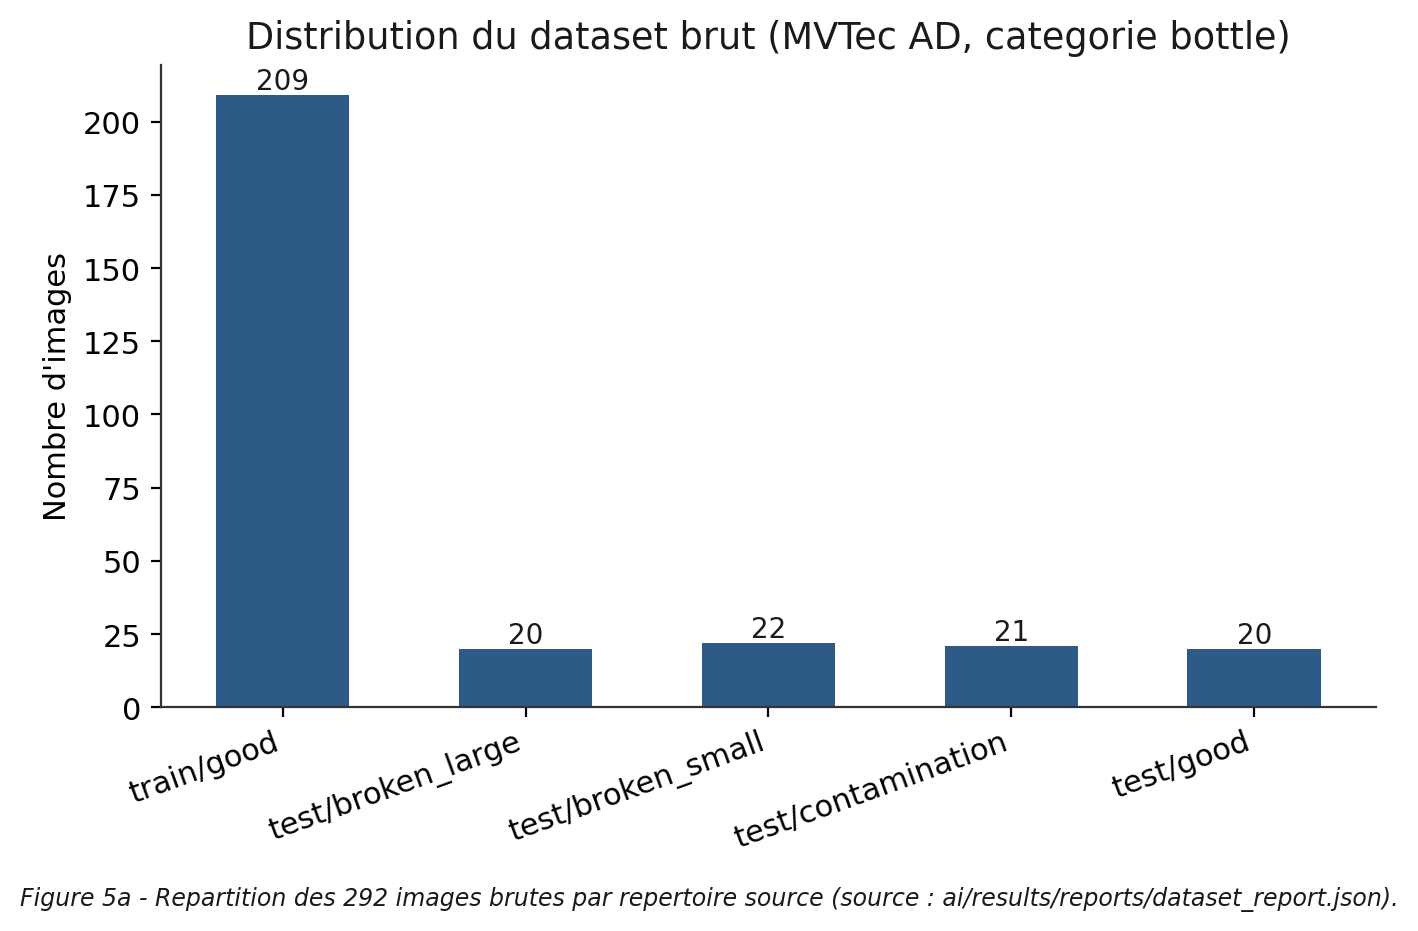
\includegraphics[width=0.85\textwidth]{figure_05a_dataset_brut.png}
\caption{Distribution du dataset brut (292 images, MVTec AD cat\'egorie bottle).}
\label{fig:dataset-brut}
\end{figure}

\section{Analyse exploratoire}

L'analyse exploratoire, r\'ealis\'ee automatiquement, a port\'e sur~:
\begin{itemize}
  \item le format des fichiers~: 292 images, toutes au format \texttt{.png}~;
  \item les dimensions~: toutes les images sont de taille homog\`ene, 900~$\times$~900~pixels~;
  \item le mode colorim\'etrique~: RGB (3 canaux) pour l'ensemble des 292 images~;
  \item l'int\'egrit\'e des fichiers~: 0 image corrompue d\'etect\'ee sur les 292 analys\'ees~;
  \item les doublons~: 0 doublon d\'etect\'e par le script d'analyse (\texttt{duplicate\_images: 0}).
\end{itemize}

\section{Nettoyage}

Le script d'analyse n'a signal\'e aucune image corrompue ni aucun doublon exact sur le jeu brut. Le nettoyage \`a ce stade s'est donc limit\'e \`a une v\'erification de conformit\'e (format, int\'egrit\'e), sans suppression d'images.

\section{V\'erification des doublons}

La v\'erification automatique des doublons exacts sur les 292 images sources n'a r\'ev\'el\'e aucune occurrence. Cette v\'erification porte sur les images brutes~; la probl\'ematique distincte de similarit\'e entre images augment\'ees (trait\'ee en \Cref{sec:data-leakage}) a n\'ecessit\'e une analyse s\'epar\'ee.

\section{R\'epartition des donn\'ees}

Compte tenu du faible nombre d'images r\'eelles disponibles par classe de d\'efaut (20 \`a 22 images), en particulier pour l'entra\^inement o\`u seules des images \texttt{good} existent nativement dans MVTec~AD, une \'etape d'augmentation a \'et\'e n\'ecessaire pour construire un jeu d'entra\^inement \'equilibr\'e entre les quatre classes.

\section{Train / Validation / Test}

Le jeu de donn\'ees a \'et\'e r\'eparti en trois ensembles disjoints (train, validation, test) avant l'\'etape d'augmentation, en veillant \`a ce qu'aucune image source ne soit partag\'ee entre plusieurs ensembles (voir \Cref{sec:data-leakage}).

\section{Redimensionnement 224$\times$224}

Toutes les images sont redimensionn\'ees en 224~$\times$~224~pixels avant d'\^etre fournies au mod\`ele, taille d'entr\'ee standard pour les architectures MobileNetV2, EfficientNetB0 et ResNet50 utilis\'ees dans ce projet (source~: \texttt{backend/app/ml/preprocessing.py}, \texttt{ai/config/config.py}).

\section{Preprocessing}

Le pipeline de pr\'etraitement, identique \`a l'entra\^inement et \`a l'inf\'erence en production, est le suivant~:
\begin{enumerate}
  \item d\'ecodage de l'image en RGB (3 canaux)~;
  \item redimensionnement bilin\'eaire en 224~$\times$~224~pixels~;
  \item conversion en \texttt{float32}, valeurs dans l'intervalle $[0, 255]$.
\end{enumerate}

La normalisation propre \`a MobileNetV2 ($x / 127{,}5 - 1{,}0$) \textbf{n'est pas appliqu\'ee \`a cette \'etape}. Elle est directement int\'egr\'ee au graphe du mod\`ele sauvegard\'e, sous la forme d'une couche personnalis\'ee \texttt{MobileNetPreprocess} (source~: \texttt{ai/models/preprocessing\_layers.py}, dupliqu\'ee dans \texttt{backend/app/ml/preprocessing\_layers.py} pour l'autonomie du backend en production --- voir \Cref{ch:deploiement}). Ce choix de conception a \'et\'e v\'erifi\'e explicitement afin d'\'eviter qu'une double normalisation ne soit appliqu\'ee \`a l'image (ce qui aurait fauss\'e les pr\'edictions).

\section{Data augmentation}

Les techniques d'augmentation r\'eellement impl\'ement\'ees dans le pipeline (source~: \path{ai/scripts/data_augmentation.py}, m\'ethode \texttt{build\_pipeline}) reposent sur les couches Keras suivantes~:
\begin{itemize}
  \item \texttt{RandomFlip} (retournement horizontal/vertical)~;
  \item \texttt{RandomRotation} (rotation al\'eatoire)~;
  \item \texttt{RandomZoom} (zoom al\'eatoire)~;
  \item \texttt{RandomBrightness} (variation al\'eatoire de luminosit\'e).
\end{itemize}

Le cahier des charges du programme mentionnait \'egalement des techniques de contraste et de recadrage (\emph{Contrast}, \emph{Crop}) parmi les augmentations possibles~; ces deux techniques sp\'ecifiques ne sont pas retrouv\'ees dans le pipeline impl\'ement\'e et ne sont donc pas revendiqu\'ees ici.

\begin{figure}[H]
\centering
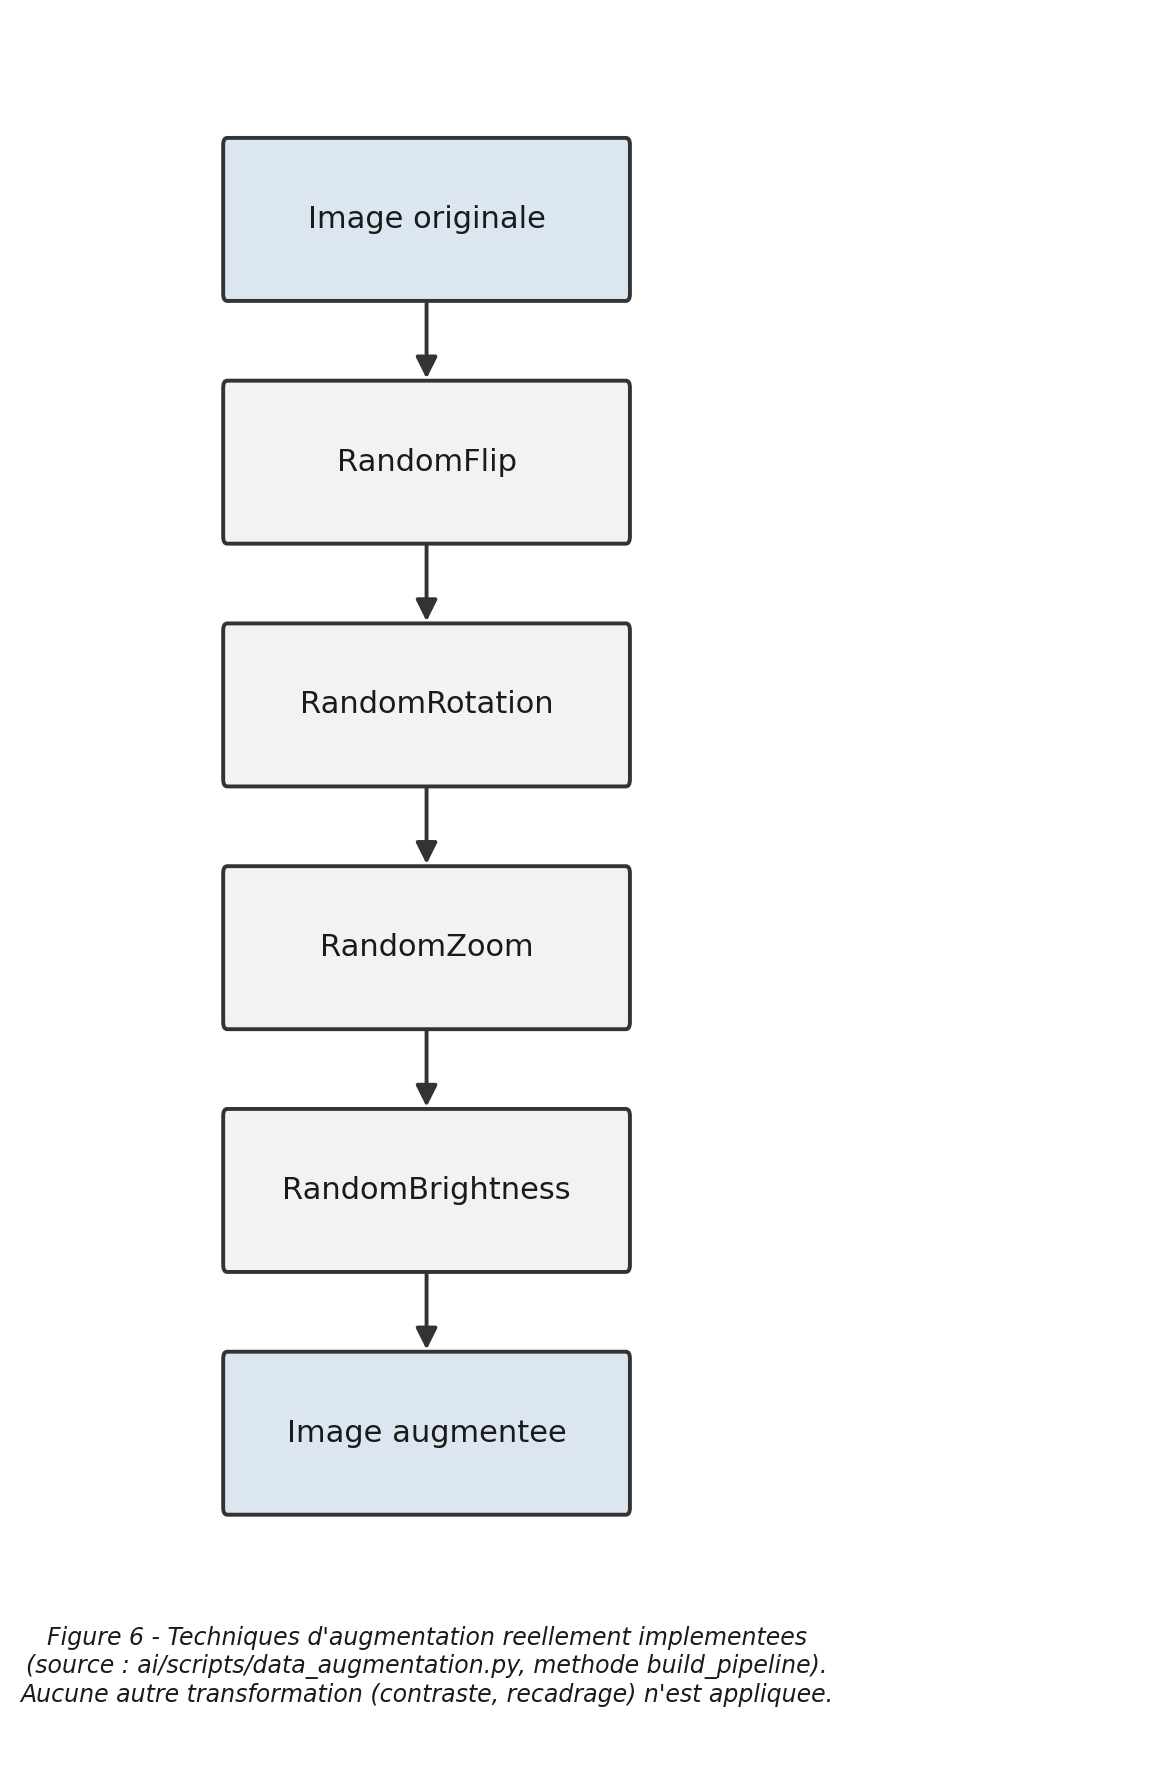
\includegraphics[width=0.55\textwidth]{figure_06_data_augmentation.png}
\caption{Techniques d'augmentation r\'eellement impl\'ement\'ees dans le pipeline.}
\label{fig:augmentation}
\end{figure}

\section{Dataset augment\'e}

L'augmentation a \'et\'e appliqu\'ee de mani\`ere diff\'erenci\'ee selon l'ensemble concern\'e~:
\begin{itemize}
  \item \textbf{Train}~: compl\'et\'e par duplication/augmentation jusqu'\`a une cible uniforme de 200 images par classe.
  \item \textbf{Test}~: compl\'et\'e de la m\^eme mani\`ere jusqu'\`a une cible de 40 images par classe.
  \item \textbf{Validation}~: trait\'e diff\'eremment par choix de conception explicite --- voir \Cref{sec:data-leakage}.
\end{itemize}

\begin{figure}[H]
\centering
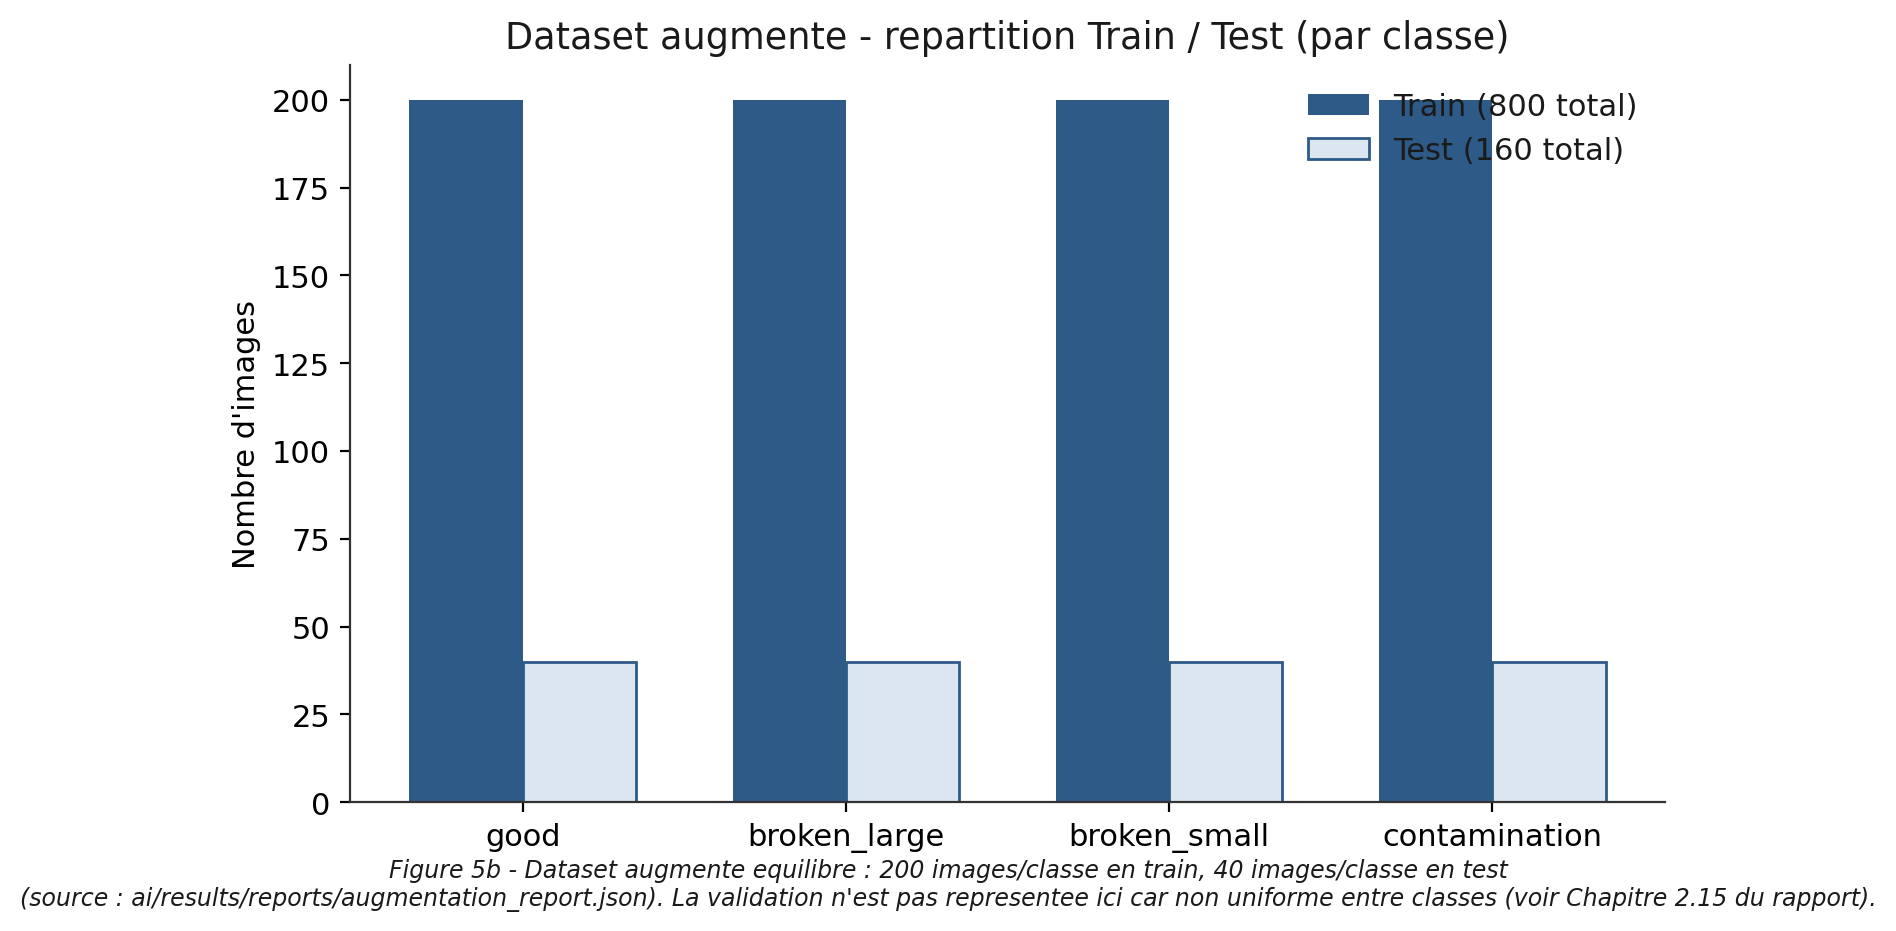
\includegraphics[width=0.85\textwidth]{figure_05b_dataset_augmente.png}
\caption{Distribution du dataset augment\'e (train/test).}
\label{fig:dataset-augmente}
\end{figure}

\section{Probl\`eme de data leakage}
\label{sec:data-leakage}

\textbf{Probl\`eme initial.} Une premi\`ere approche consistait \`a compl\'eter (\guillemotleft~padder~\guillemotright) l'ensemble de validation par duplication, \`a l'instar de l'ensemble de test, afin d'atteindre un nombre cible uniforme d'images par classe.

\textbf{D\'etection du probl\`eme.} Cette approche a \'et\'e identifi\'ee comme risqu\'ee~: un signal de validation bas\'e sur des images dupliqu\'ees (quasi identiques \`a des images du jeu d'entra\^inement apr\`es augmentation) est bruit\'e et peut fausser les d\'ecisions prises pendant l'entra\^inement sur la base de ce signal, en particulier l'\emph{early stopping} et la s\'election du meilleur point de sauvegarde (\emph{checkpoint}) du mod\`ele. Cette analyse est document\'ee explicitement dans le code source (\texttt{ai/scripts/data\_augmentation.py}, m\'ethode \texttt{balance\_split})~:

\begin{quote}
\itshape \guillemotleft~pad=False~: contrairement au test, la validation n'est jamais compl\'et\'ee par des copies dupliqu\'ees. Un signal de validation bas\'e sur des doublons est bruit\'e et fausse les d\'ecisions d'early stopping / s\'election du meilleur checkpoint pendant l'entra\^inement. On garde donc uniquement les images r\'eelles uniques disponibles, quitte \`a avoir moins que la cible.~\guillemotright
\end{quote}

\textbf{Correction appliqu\'ee.} L'ensemble de validation est donc construit exclusivement \`a partir d'images r\'eelles uniques, sans compl\'etion par duplication, quitte \`a obtenir un nombre d'images inf\'erieur \`a la cible nominale de 40 par classe pour les classes disposant de peu d'images sources.

\textbf{Protocole final.} Le jeu de test, en revanche, est compl\'et\'e par duplication pour atteindre 40 images par classe de fa\c{c}on homog\`ene, ce choix \'etant jug\'e acceptable dans la mesure o\`u le test n'intervient pas dans les d\'ecisions prises pendant l'entra\^inement.

\textbf{Preuve indirecte de la correction.} Le d\'ep\^ot conserve plusieurs \emph{runs} exp\'erimentaux de MobileNetV2 permettant de tracer cette \'evolution~:
\begin{itemize}
  \item \texttt{ai/results/mobilenet\_v2\_baseline\_padded\_val/} (09/08/2026, 02:16)~: validation compos\'ee de 160 images (40 par classe --- coh\'erent avec une validation \emph{padd\'ee})~;
  \item \texttt{ai/results/mobilenet\_v2\_exp0\_fixed\_val/} (09/08/2026, 17:06)~: validation r\'eduite \`a 64 images (\emph{fixed\_val}, coh\'erent avec la correction d\'ecrite ci-dessus)~;
  \item \texttt{ai/results/mobilenet\_v2/} (run final retenu, 09/08/2026, 17:18)~: validation \'egalement compos\'ee de 64 images, confirmant que le mod\`ele retenu a bien \'et\'e entra\^in\'e selon le protocole corrig\'e.
\end{itemize}

\section{Dataset final}

\begin{table}[H]
\centering
\caption{R\'epartition Train / Validation / Test (dataset augment\'e)}
\label{tab:dataset-final}
\begin{tabular}{lrl}
\toprule
Ensemble & Images totales & Par classe (cible) \\
\midrule
Train & 800 & 200 \\
Test & 160 & 40 \\
Validation & 64 (mod\`ele retenu) & non uniforme, voir ci-dessous \\
\bottomrule
\end{tabular}
\end{table}

\begin{noteflag}{Incoh\'erence \`a v\'erifier}
Le fichier \texttt{ai/results/reports/augmentation\_report.json} (g\'en\'er\'e le 09/08/2026 \`a 17:13) rapporte une composition de validation de \textbf{55 images} (40 pour \texttt{good}, 5 pour chacune des trois classes de d\'efaut), alors que le fichier \texttt{training\_report.json} du mod\`ele MobileNetV2 finalement retenu (g\'en\'er\'e \`a 17:18, soit peu apr\`es) indique \textbf{64 images} de validation. L'\'ecart de 9 images entre ces deux fichiers, g\'en\'er\'es \`a quelques minutes d'intervalle, n'a pas pu \^etre expliqu\'e \`a partir des fichiers disponibles dans le d\'ep\^ot~; il est possible qu'une r\'eg\'en\'eration partielle du split de validation soit intervenue entre les deux ex\'ecutions. Cette incoh\'erence est signal\'ee ici plut\^ot que r\'esolue arbitrairement.
\end{noteflag}

Toutes les architectures compar\'ees au \Cref{ch:modelisation} n'ont pas n\'ecessairement \'et\'e entra\^in\'ees avec la m\^eme taille de validation~: les \emph{runs} de ResNet50, EfficientNetB0, CNN et CNN am\'elior\'e rapportent chacun 160 images de validation, contre 64 pour le run MobileNetV2 finalement retenu. Cette diff\'erence de protocole entre mod\`eles compar\'es constitue une limite du benchmark, discut\'ee au \Cref{ch:discussion}.

\chapter{Mod\'elisation IA}
\label{ch:modelisation}

\section{Probl\`eme de classification}

Il s'agit d'un probl\`eme de classification d'images multi-classes (4~classes), \`a sortie unique (chaque image appartient \`a exactement une classe).

\section{CNN de base}

Un r\'eseau de neurones convolutif (CNN) construit et entra\^in\'e int\'egralement \`a partir de z\'ero (sans poids pr\'e-entra\^in\'es) a \'et\'e inclus dans la comparaison, afin de disposer d'une r\'ef\'erence (\emph{baseline}) ne b\'en\'eficiant d'aucun transfert de connaissances.

\section{Transfer learning}

Les trois autres architectures compar\'ees (MobileNetV2, EfficientNetB0, ResNet50) exploitent le \emph{transfer learning}~: un backbone pr\'e-entra\^in\'e sur ImageNet est r\'eutilis\'e, gel\'e (\texttt{trainable=False}), seule une t\^ete de classification ajout\'ee en sortie \'etant entra\^in\'ee sur le dataset \emph{bottle} (protocole dit de \emph{feature extraction}).

\section{MobileNetV2}

Architecture l\'eg\`ere, fond\'ee sur des convolutions s\'eparables en profondeur (\emph{depthwise separable convolutions}), initialement con\c{c}ue pour des d\'eploiements mobiles/embarqu\'es. Retenue au final pour ce projet (justification d\'etaill\'ee en \Cref{sec:selection-mobilenet})~\cite{mobilenetv2}.

\section{EfficientNetB0}

Architecture fond\'ee sur un principe de \emph{compound scaling} (mise \`a l'\'echelle simultan\'ee de la profondeur, de la largeur et de la r\'esolution du r\'eseau), incluse dans la comparaison~\cite{efficientnet}.

\section{ResNet50}

Architecture \`a connexions r\'esiduelles, plus profonde et plus lourde que les deux pr\'ec\'edentes (23,6~millions de param\`etres contre 2,26~pour MobileNetV2), \'egalement incluse dans la comparaison~\cite{resnet}.

\section{M\'ethodologie d'entra\^inement}

\begin{table}[H]
\centering
\caption{Hyperparam\`etres d'entra\^inement}
\label{tab:hyperparams}
\begin{tabular}{lll}
\toprule
Param\`etre & MobileNetV2 / ResNet50 / EffNetB0 & CNN / CNN am\'elior\'e \\
\midrule
\'Epoques (max.) & 30 & 30 \\
Taille de batch & 32 & 32 \\
Taux d'apprentissage & 0,001 & 0,001 \\
Optimiseur & Adam & AdamW \\
Dropout & 0,3 & 0,3 \\
Weight decay & 0,0001 & 0,0001 \\
Taille d'image & 224$\times$224 & 224$\times$224 \\
Nombre de classes & 4 & 4 \\
Graine al\'eatoire (seed) & 42 & 42 \\
\bottomrule
\end{tabular}
\end{table}

\section{Fonction de perte}

\texttt{SparseCategoricalCrossentropy}, utilis\'ee de fa\c{c}on identique pour les quatre architectures (source~: \texttt{ai/models/mobilenet\_model.py}, \texttt{resnet\_model.py}, \texttt{efficientnet\_model.py}, \texttt{cnn\_model.py}).

\section{Optimiseur}

Adam pour MobileNetV2, ResNet50 et EfficientNetB0~; AdamW pour le CNN personnalis\'e et sa variante am\'elior\'ee.

\section{Callbacks}

\begin{itemize}
  \item \textbf{EarlyStopping}~: patience de 8~\'epoques, surveillance de \texttt{val\_loss}~;
  \item \textbf{ModelCheckpoint}~: sauvegarde du meilleur mod\`ele selon \texttt{val\_loss} (\texttt{save\_best\_only=True}).
\end{itemize}

\section{\'Evaluation}

Les m\'etriques calcul\'ees pour chaque mod\`ele sur le jeu de test sont~: accuracy, precision macro, recall macro, F1-score macro, ainsi qu'une matrice de confusion.

\begin{noteflag}{Donn\'ee non v\'erifiable}
Le cahier des charges demande \'egalement une courbe ROC par mod\`ele~; aucun fichier correspondant \`a une courbe ROC n'a \'et\'e retrouv\'e dans \texttt{ai/results/}. Cette visualisation n'a donc pas pu \^etre produite dans le cadre de ce rapport.
\end{noteflag}

\section{Benchmark}

\begin{table}[H]
\centering
\small
\caption{Benchmark comparatif des mod\`eles (jeu de test, 160~images, 40 par classe)}
\label{tab:benchmark}
\begin{tabularx}{\textwidth}{lrrrrrrr}
\toprule
Mod\`ele & Acc. & Prec. & Rec. & F1 & Taille & T. entra\^in. & Inf\'erence \\
\midrule
\textbf{MobileNetV2 (retenu)} & \textbf{75,63\,\%} & \textbf{0,839} & \textbf{0,756} & \textbf{0,742} & \textbf{9,24\,Mo} & \textbf{3\,min\,57\,s} & \textbf{9,16\,ms} \\
ResNet50 & 78,13\,\% & 0,818 & 0,781 & 0,772 & 90,71\,Mo & 10\,min\,17\,s & 23,70\,ms \\
EfficientNetB0 & 71,25\,\% & 0,826 & 0,713 & 0,688 & 16,32\,Mo & 5\,min\,56\,s & 11,45\,ms \\
CNN (from scratch) & 25,00\,\% & 0,063 & 0,250 & 0,100 & 21,68\,Mo & $\approx$8\,min\,40\,s & 7,4--7,8\,ms \\
\bottomrule
\end{tabularx}
\end{table}

\begin{noteflag}{Incoh\'erence \`a v\'erifier}
Le fichier \texttt{ai/results/benchmark\_results.json} comporte, pour chaque mod\`ele, un champ \texttt{accuracy} de premier niveau dont la valeur ne correspond pas \`a celle du fichier \texttt{classification\_report.json} du m\^eme mod\`ele (exemple~: 99,37\,\% pour MobileNetV2 dans \texttt{benchmark\_results.json}, contre 75,63\,\% dans \texttt{classification\_report.json}, ce dernier \'etant coh\'erent avec le F1-score macro rapport\'e de 0,742). Cette incoh\'erence a \'et\'e r\'esolue en retenant les valeurs de \texttt{classification\_report.json} comme r\'ef\'erence, celles-ci \'etant seules coh\'erentes en interne avec les autres m\'etriques macro rapport\'ees.
\end{noteflag}

\textbf{R\'esultat d'un benchmark ant\'erieur, sur dataset non augment\'e.} Un premier benchmark (\texttt{ai/results/benchmark\_report.md}, dat\'e du 08/08/2026), r\'ealis\'e sur le dataset brut de 292~images (avant la construction du dataset augment\'e \'equilibr\'e), avait donn\'e des r\'esultats tr\`es d\'egrad\'es et strictement identiques pour les quatre architectures (F1-score macro de 0,2179 pour chacune), le rapport concluant \`a un sous-apprentissage g\'en\'eralis\'e li\'e \`a l'insuffisance de donn\'ees et au protocole de \emph{feature extraction} \`a backbone gel\'e sur un jeu de donn\'ees aussi r\'eduit. Ce benchmark constitue une it\'eration interm\'ediaire du projet, corrig\'ee par la suite via la construction du dataset augment\'e \'equilibr\'e, et n'est pas repr\'esentatif de la performance du mod\`ele finalement int\'egr\'e \`a l'application.

\begin{table}[H]
\centering
\caption{Classification report d\'etaill\'e (MobileNetV2, mod\`ele retenu)}
\label{tab:classification-report}
\begin{tabular}{lrrrr}
\toprule
Classe & Precision & Recall & F1-score & Support \\
\midrule
\texttt{broken\_large} & 0,741 & 1,000 & 0,851 & 40 \\
\texttt{broken\_small} & 1,000 & 0,500 & 0,667 & 40 \\
\texttt{contamination} & 1,000 & 0,525 & 0,689 & 40 \\
\texttt{good} & 0,615 & 1,000 & 0,762 & 40 \\
\bottomrule
\end{tabular}
\end{table}

\begin{figure}[H]
\centering
\begin{subfigure}[b]{0.48\textwidth}
  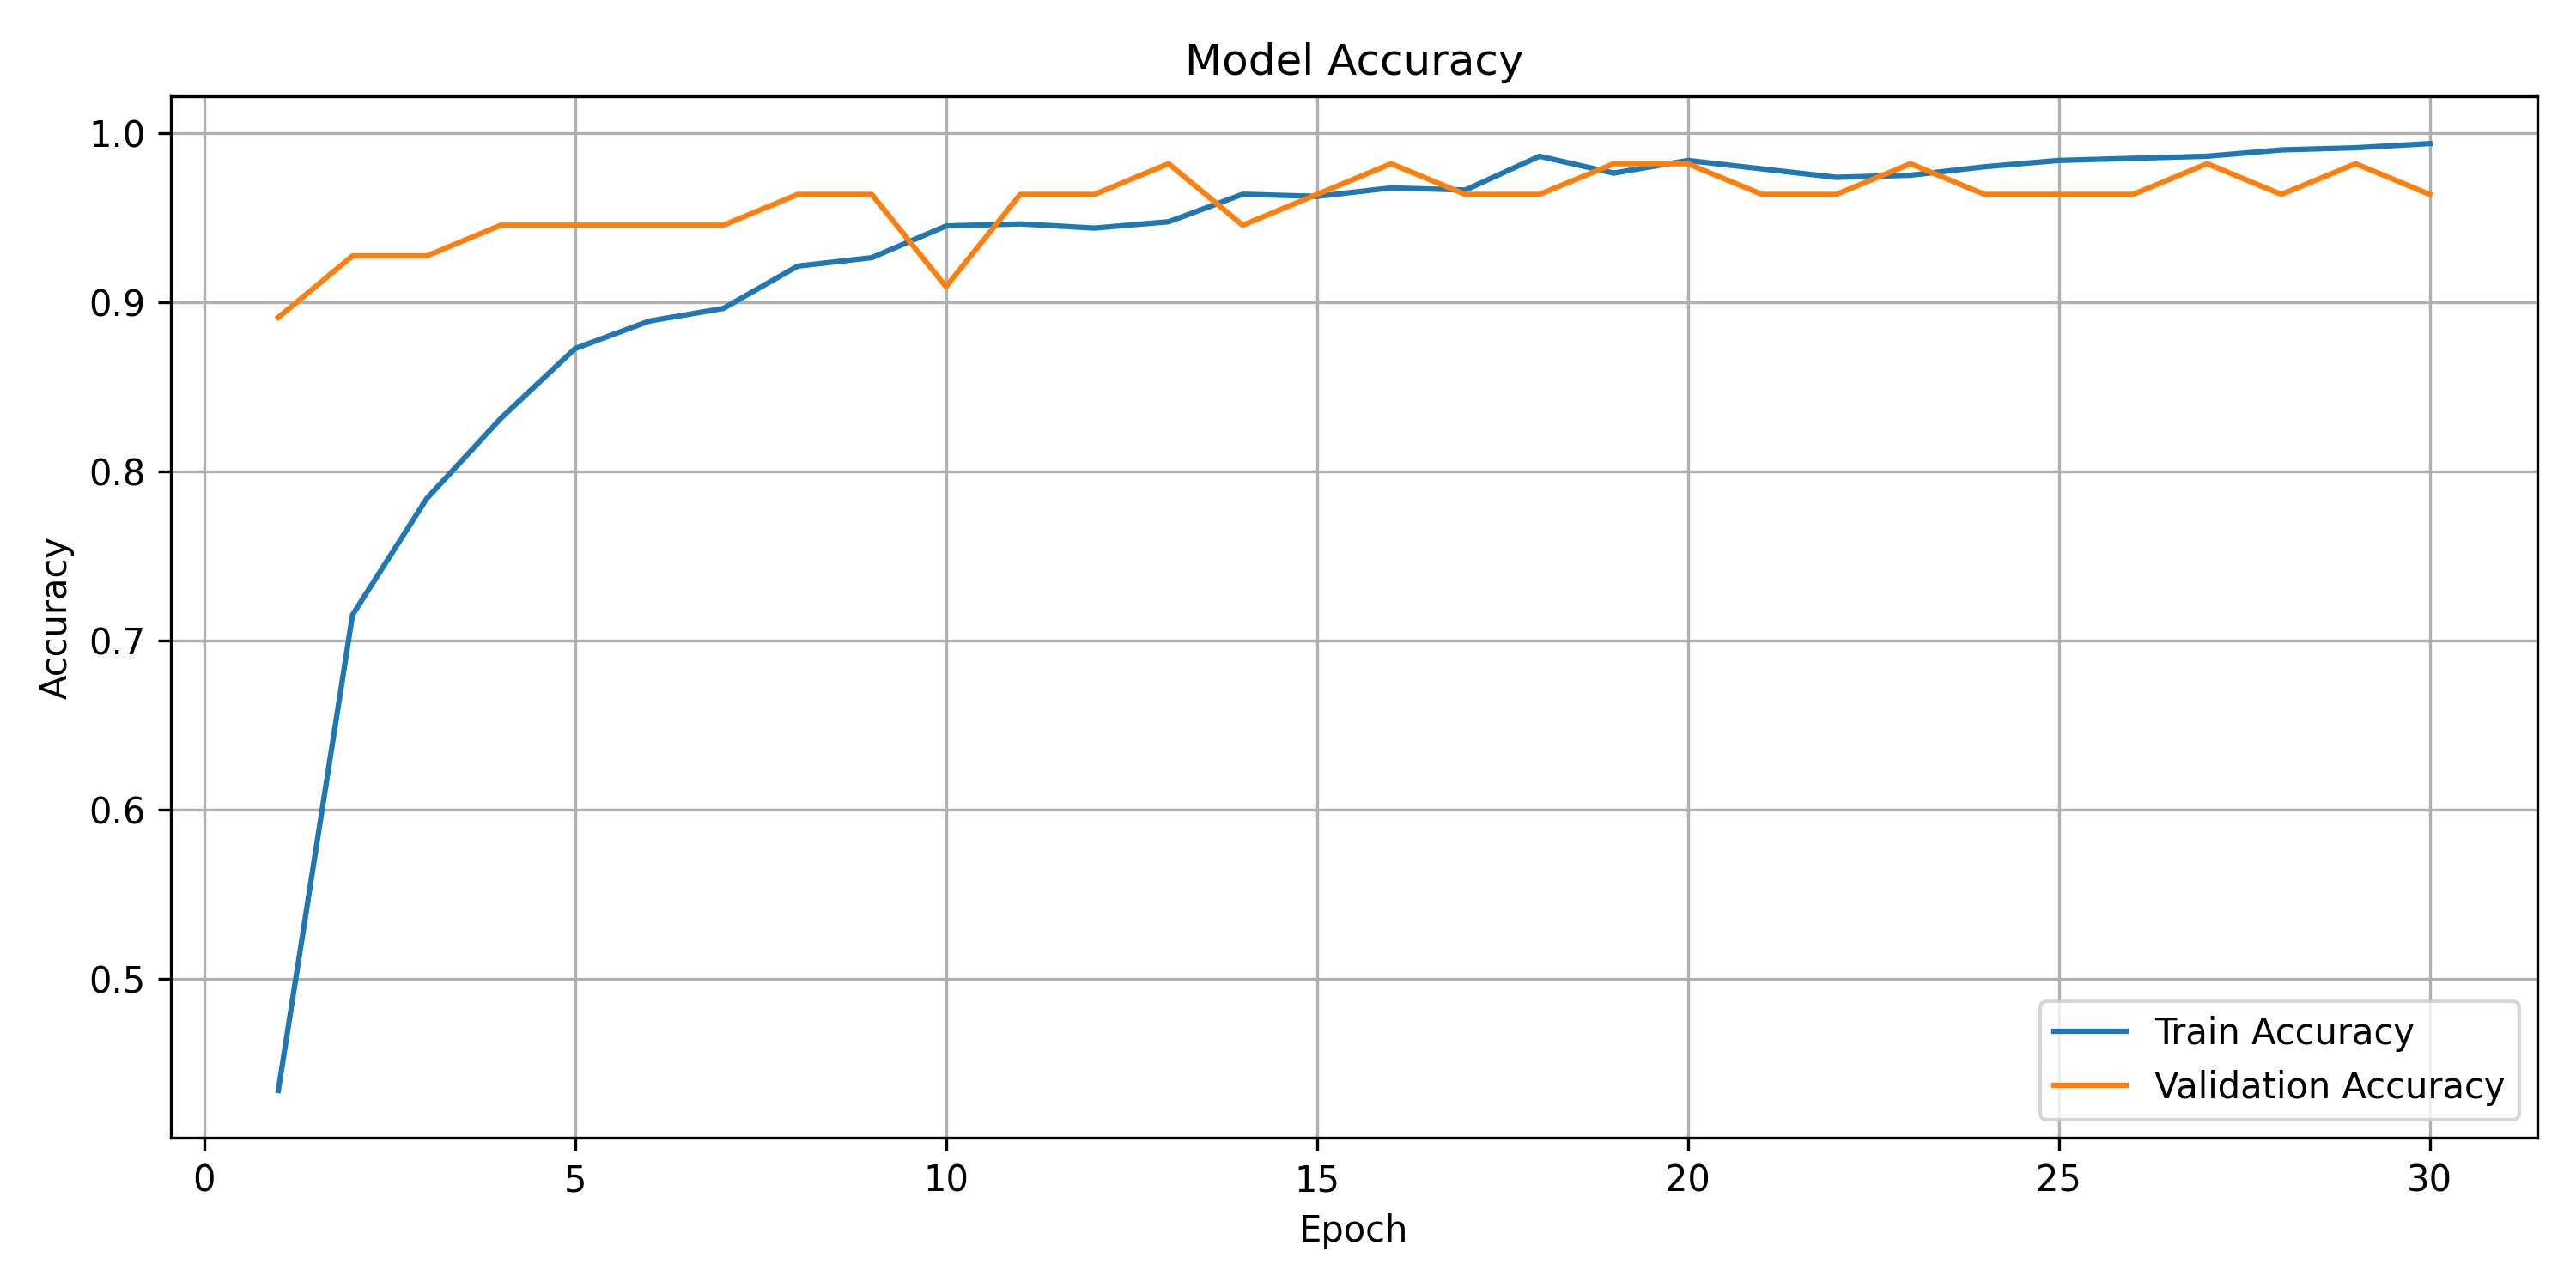
\includegraphics[width=\textwidth]{figure_07_accuracy_training.png}
  \caption{Accuracy pendant l'entra\^inement}
\end{subfigure}
\hfill
\begin{subfigure}[b]{0.48\textwidth}
  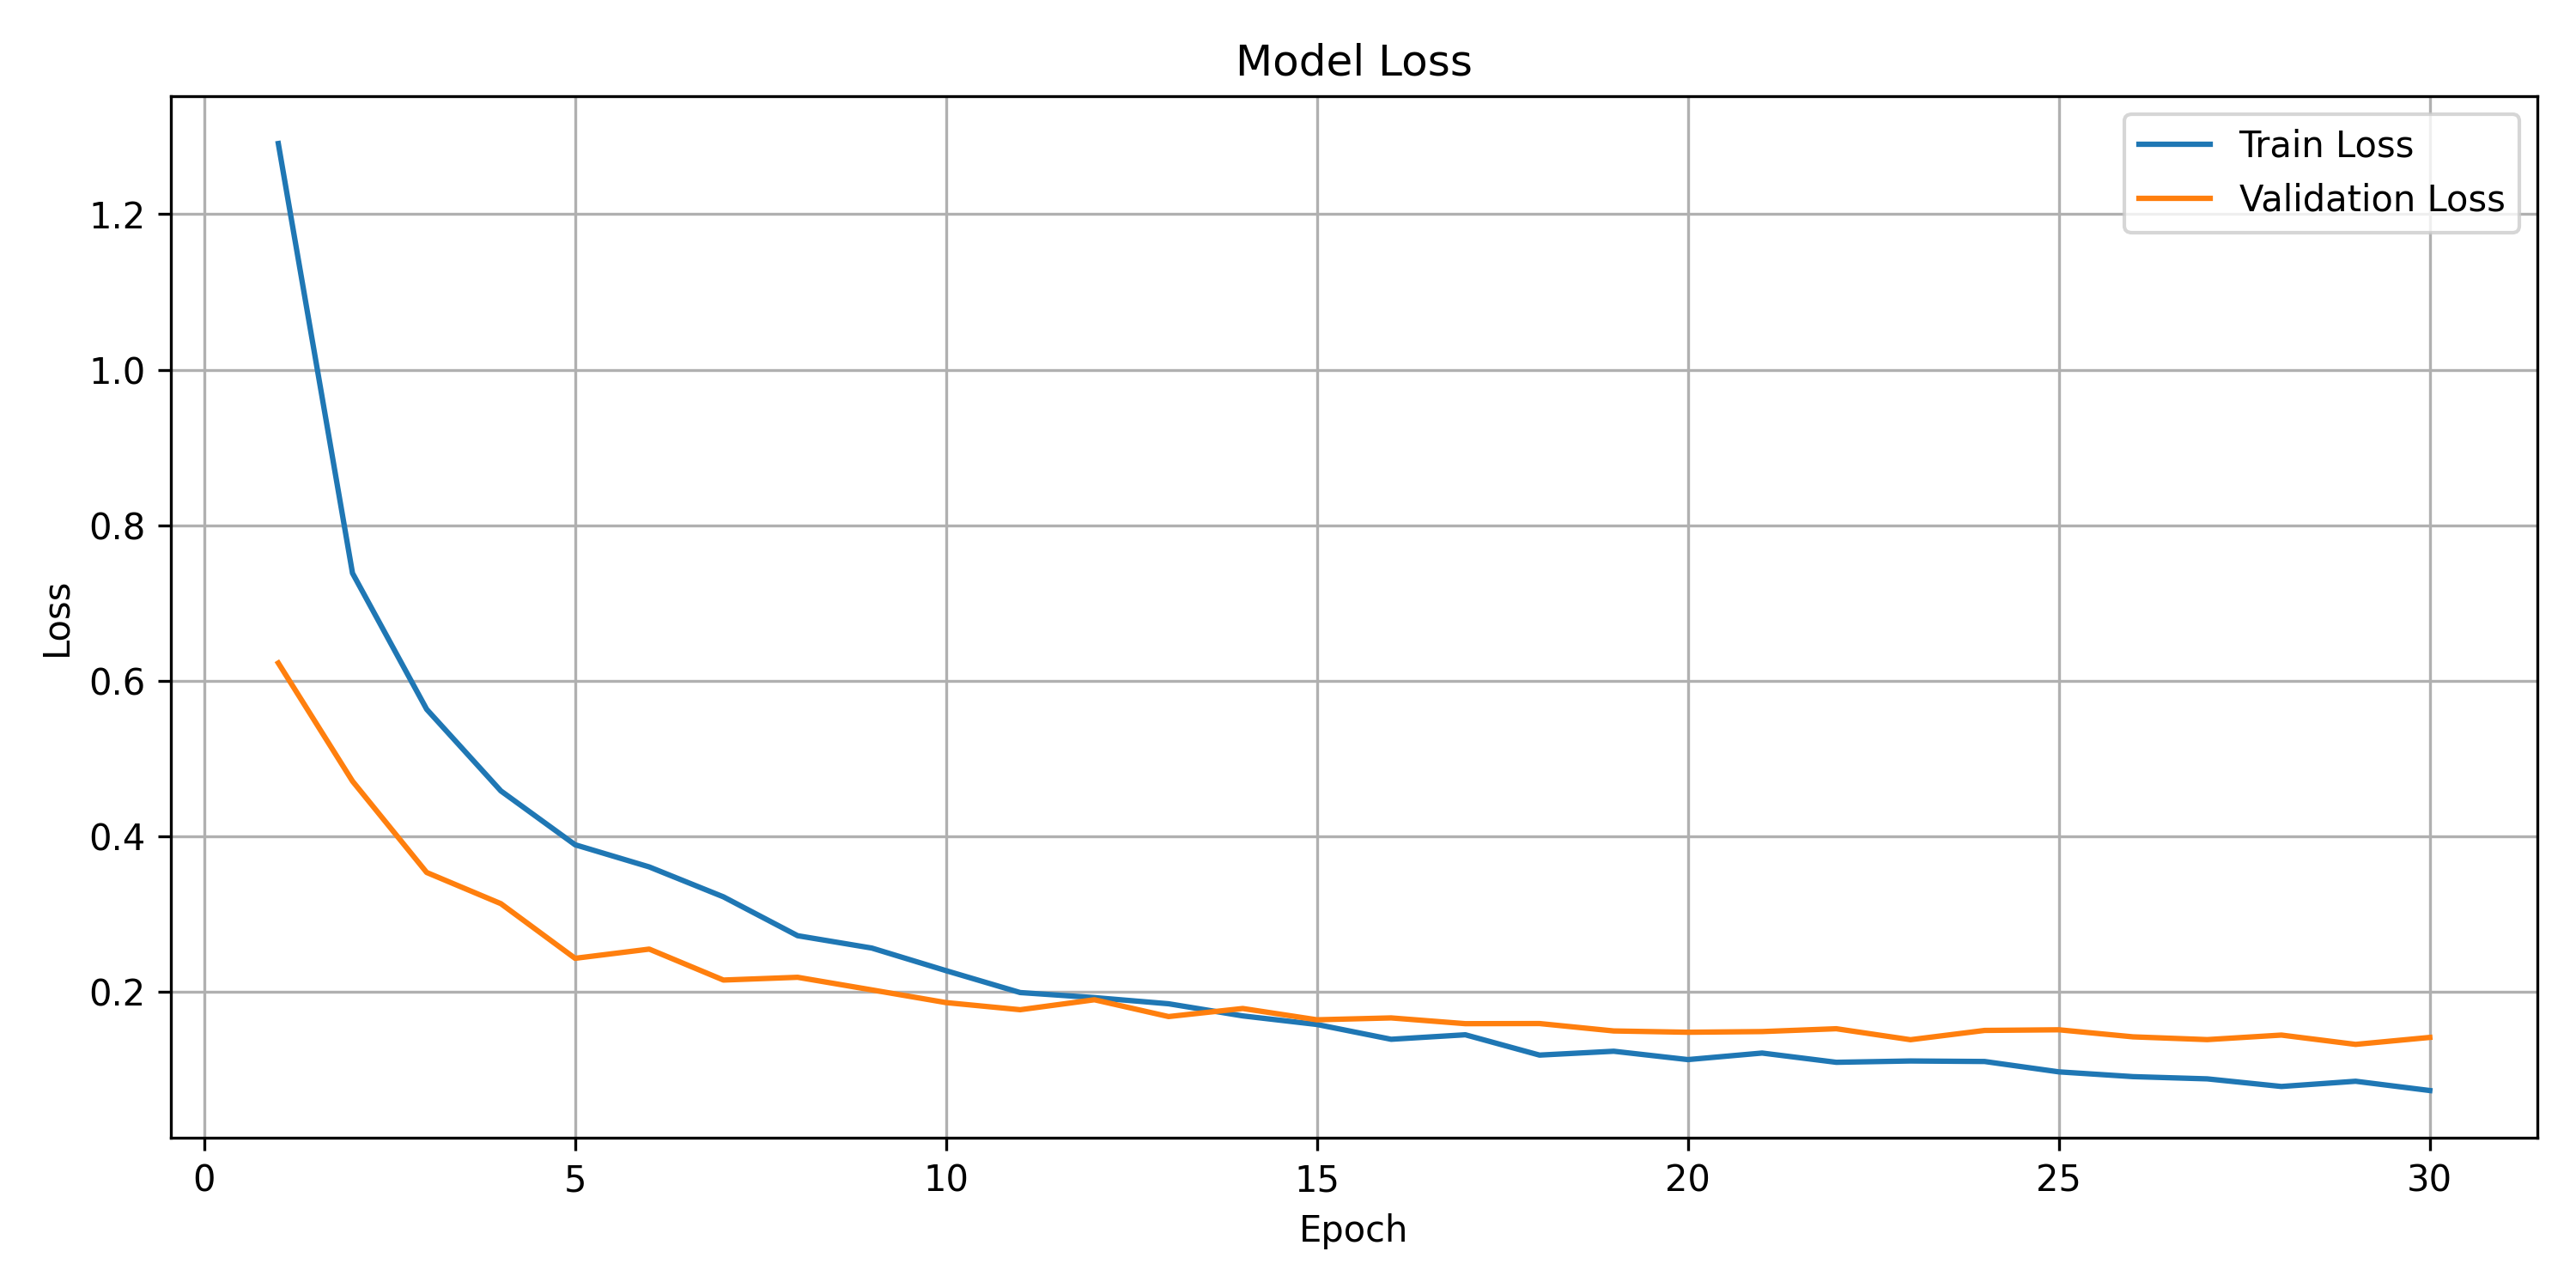
\includegraphics[width=\textwidth]{figure_08_loss_training.png}
  \caption{Loss pendant l'entra\^inement}
\end{subfigure}
\caption{Courbes d'entra\^inement de MobileNetV2 (source~: \texttt{ai/results/mobilenet\_v2/}).}
\label{fig:courbes-entrainement}
\end{figure}

\begin{figure}[H]
\centering
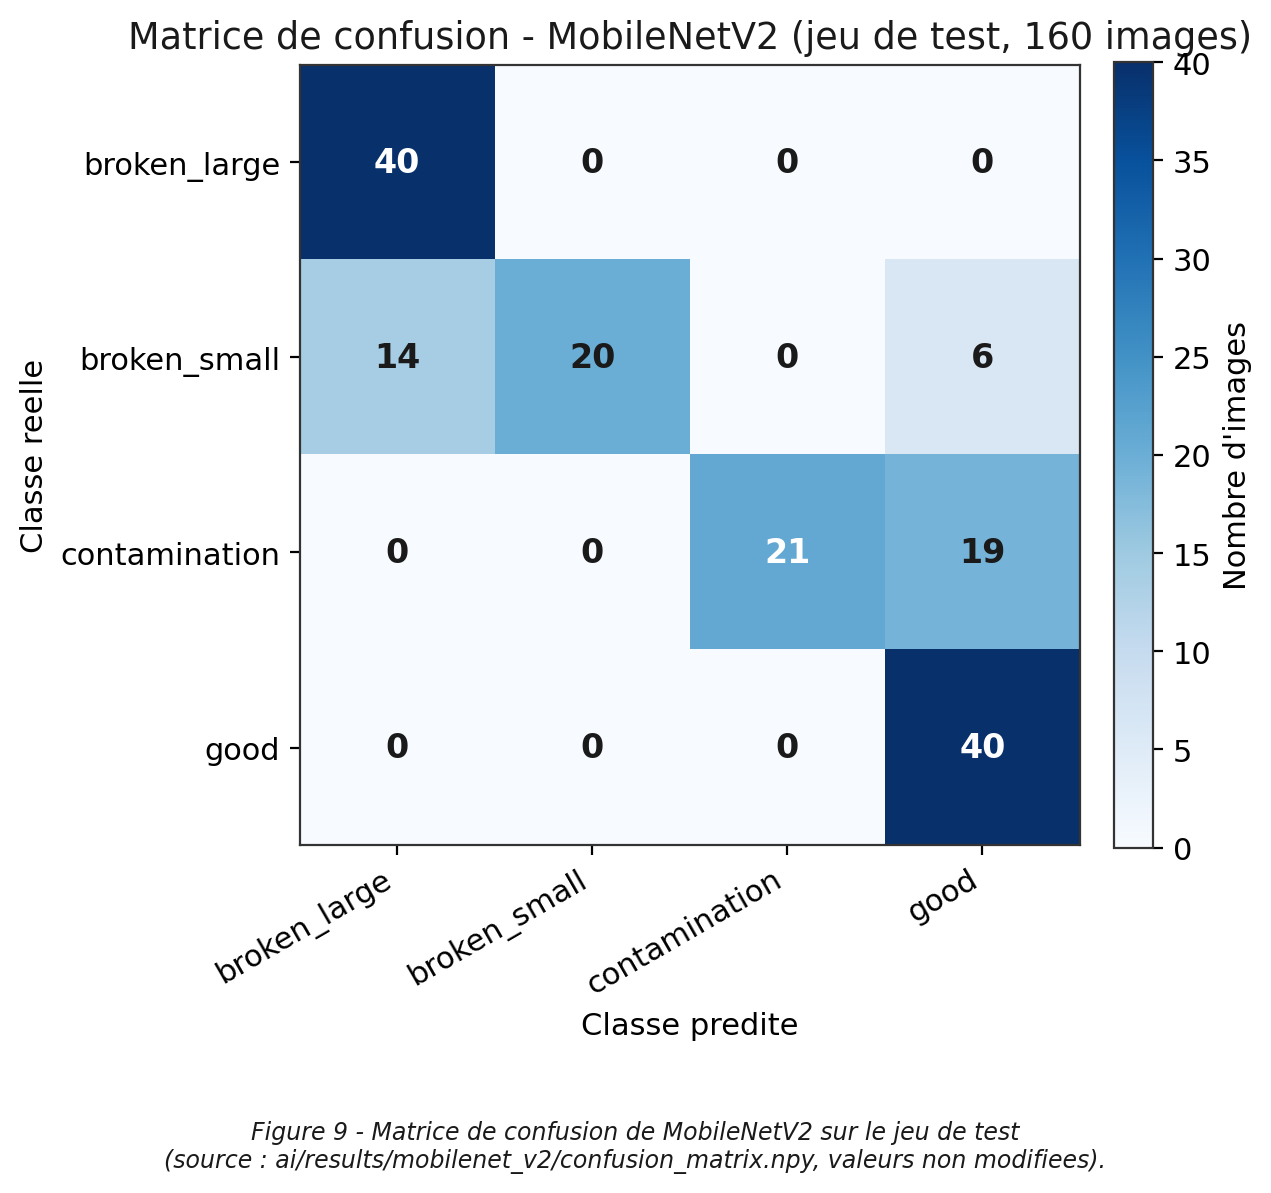
\includegraphics[width=0.65\textwidth]{figure_09_matrice_confusion.png}
\caption{Matrice de confusion de MobileNetV2 sur le jeu de test.}
\label{fig:confusion-matrix}
\end{figure}

\begin{figure}[H]
\centering
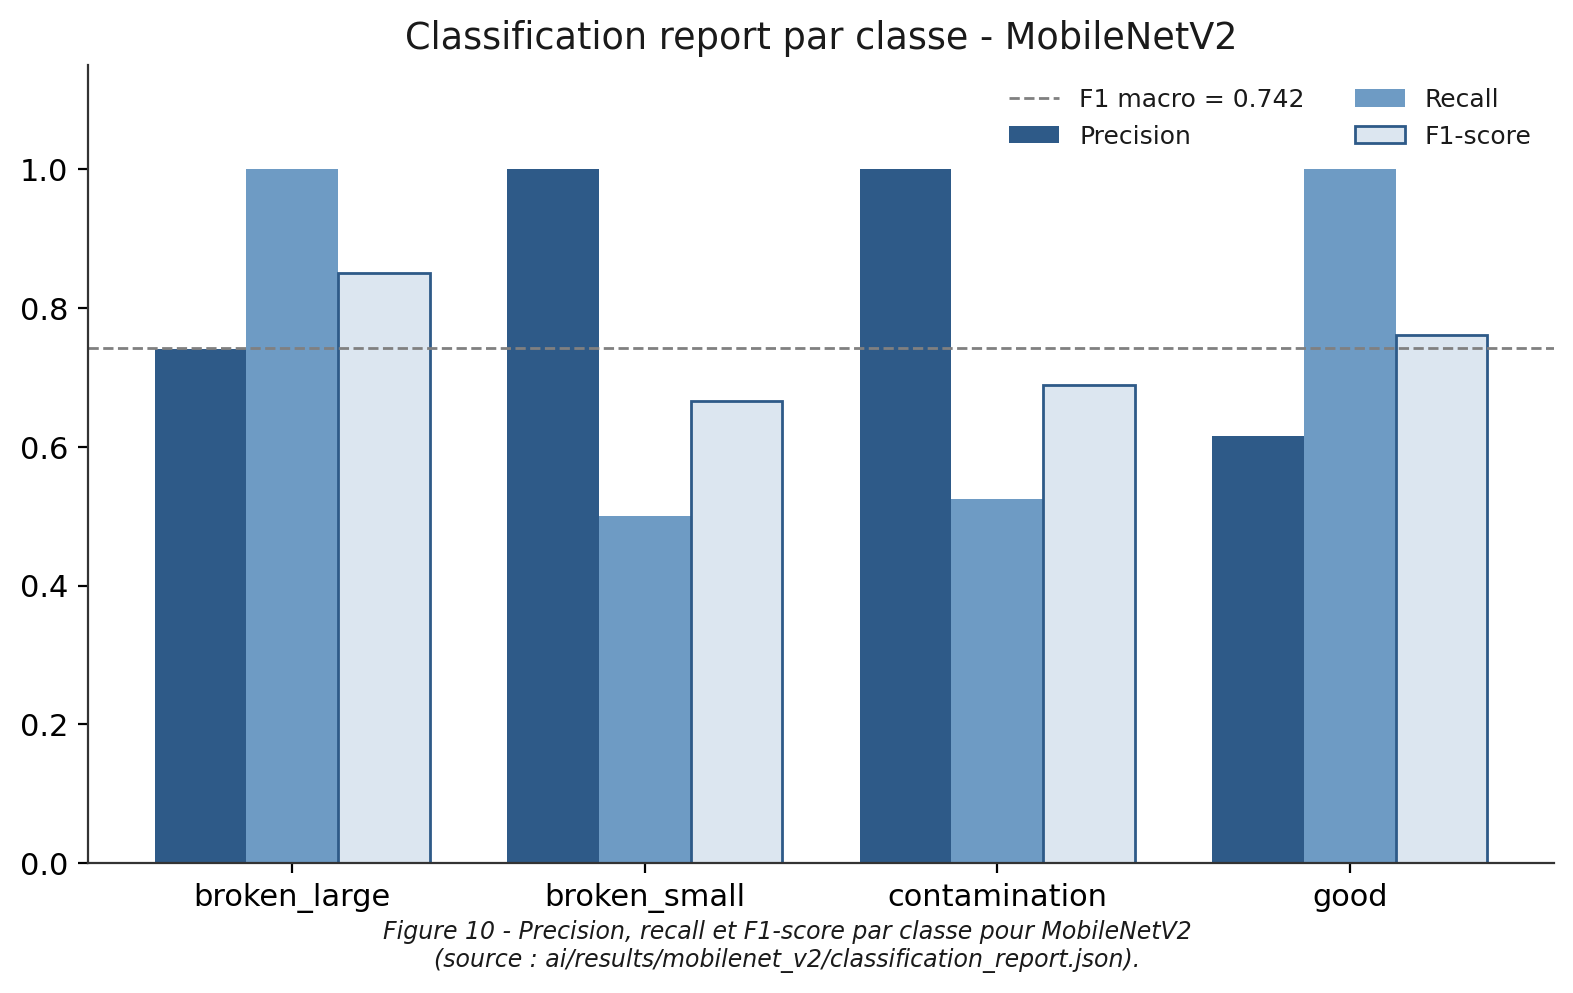
\includegraphics[width=0.8\textwidth]{figure_10_classification_report.png}
\caption{Precision, recall et F1-score par classe pour MobileNetV2.}
\label{fig:classification-report-fig}
\end{figure}

\begin{figure}[H]
\centering
\begin{subfigure}[b]{0.32\textwidth}
  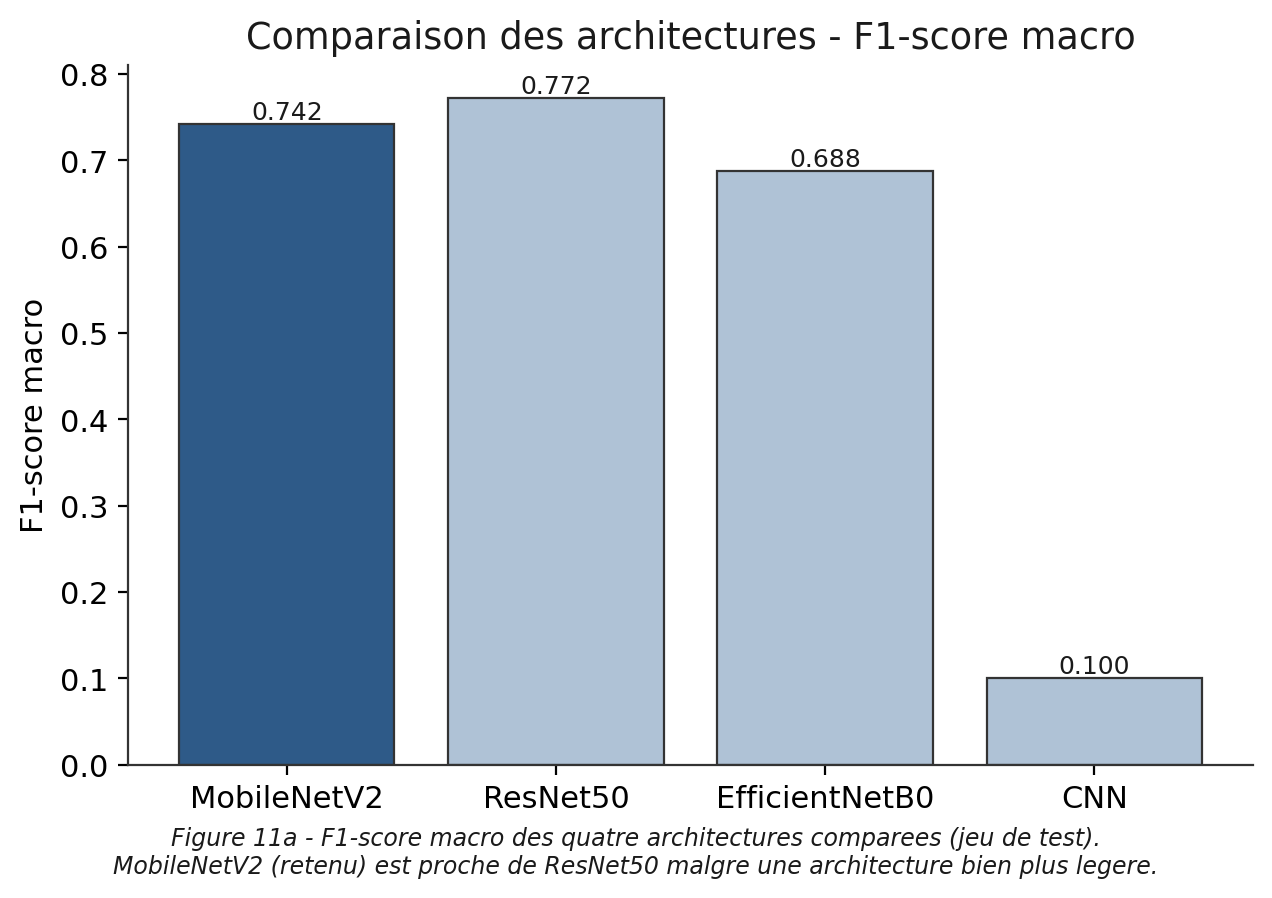
\includegraphics[width=\textwidth]{figure_11a_comparaison_f1.png}
\end{subfigure}
\hfill
\begin{subfigure}[b]{0.32\textwidth}
  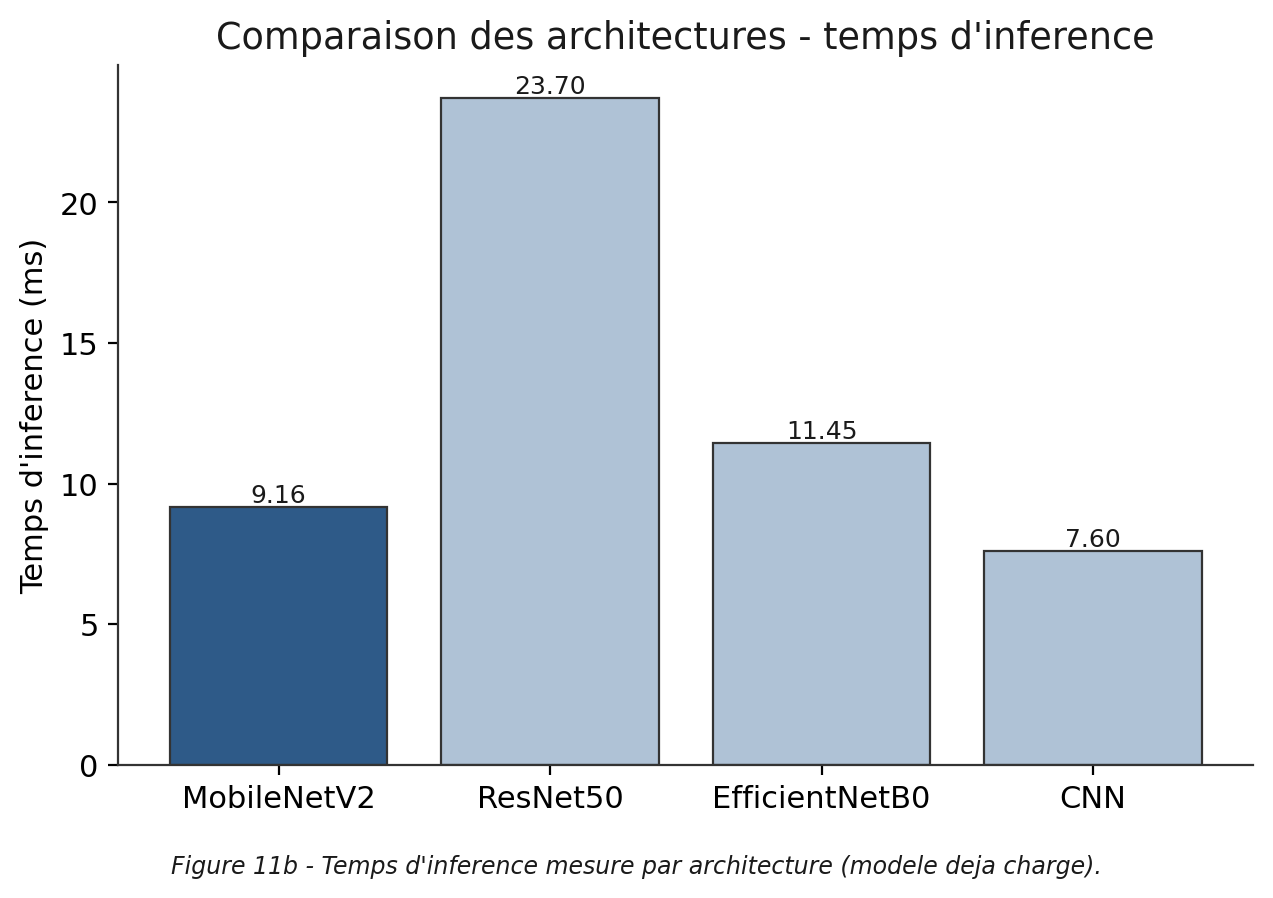
\includegraphics[width=\textwidth]{figure_11b_comparaison_inference.png}
\end{subfigure}
\hfill
\begin{subfigure}[b]{0.32\textwidth}
  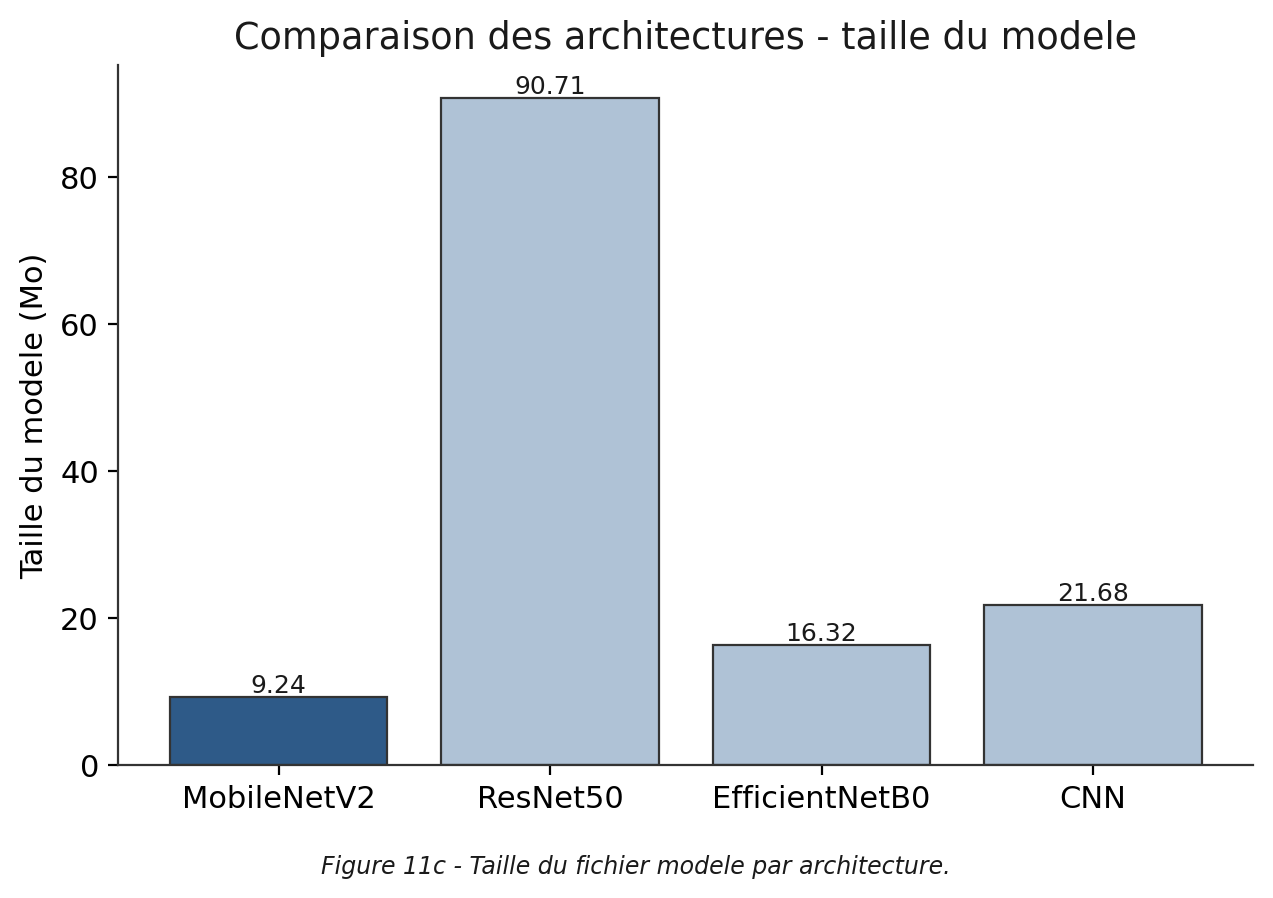
\includegraphics[width=\textwidth]{figure_11c_comparaison_taille.png}
\end{subfigure}
\caption{Comparaison des quatre architectures~: F1-score macro, temps d'inf\'erence, taille du mod\`ele.}
\label{fig:comparaison-modeles}
\end{figure}

\section{Analyse des r\'esultats}

Les trois mod\`eles pr\'e-entra\^in\'es sur ImageNet (MobileNetV2, EfficientNetB0, ResNet50) surpassent nettement le CNN entra\^in\'e \`a partir de z\'ero, dont l'accuracy (25\,\%) reste proche du niveau du hasard pour un probl\`eme \`a quatre classes \'equilibr\'ees, ce qui met en \'evidence l'apport du transfer learning dans un contexte de donn\'ees limit\'ees.

Entre les trois mod\`eles pr\'e-entra\^in\'es, ResNet50 obtient l'accuracy la plus \'elev\'ee (78,13\,\% contre 75,63\,\% pour MobileNetV2), mais cet \'ecart de 2,5~points doit \^etre interpr\'et\'e avec prudence~: le jeu de test ne comporte que quelques images sources r\'eellement uniques par classe (le reste \'etant obtenu par duplication/augmentation), ce qui limite la robustesse statistique d'un tel \'ecart.

Le \Cref{tab:classification-report} met en \'evidence un comportement diff\'erenci\'e selon les classes pour MobileNetV2~: un rappel parfait (1,0) sur \texttt{broken\_large} et \texttt{good}, mais un rappel faible (0,5 et 0,525) sur \texttt{broken\_small} et \texttt{contamination}, ces deux classes \'etant plus difficiles \`a distinguer visuellement dans ce dataset.

\section{S\'election de MobileNetV2}
\label{sec:selection-mobilenet}

Dans les conditions exp\'erimentales de ce projet, \textbf{MobileNetV2 a \'et\'e retenu comme meilleur compromis entre performance, taille du mod\`ele et temps d'inf\'erence}, plut\^ot que comme le mod\`ele objectivement le plus performant~:
\begin{itemize}
  \item \textbf{Performance}~: F1-score macro de 0,742, proche de celui de ResNet50 (0,772) et sup\'erieur \`a celui d'EfficientNetB0 (0,688).
  \item \textbf{Taille du mod\`ele}~: 9,24~Mo, soit environ 10~fois plus l\'eger que ResNet50 (90,71~Mo).
  \item \textbf{Rapidit\'e d'inf\'erence}~: environ 9~ms, soit 2,6~fois plus rapide que ResNet50 (23,70~ms).
  \item \textbf{Facilit\'e de d\'eploiement}~: ces caract\'eristiques rendent le mod\`ele mieux adapt\'e \`a une int\'egration dans une application web sans infrastructure GPU d\'edi\'ee (voir \Cref{ch:deploiement}).
\end{itemize}

\section{Mod\`ele final}

Le mod\`ele final retenu est sauvegard\'e au format natif Keras~3 (\texttt{.keras})~: \path{ai/saved_models/mobilenet_v2/best_model.keras}. Une copie de ce m\^eme fichier (identit\'e v\'erifi\'ee par empreinte SHA-256, voir \Cref{ch:deploiement}) est int\'egr\'ee au backend pour les besoins du d\'eploiement.

\begin{noteflag}{Incoh\'erence \`a v\'erifier}
Le cahier des charges demande explicitement un export au format \texttt{.h5} ou \texttt{.pt}. Le projet utilise le format \texttt{.keras} (format natif de Keras~3, successeur recommand\'e du format \texttt{.h5} par la biblioth\`eque elle-m\^eme), ni \texttt{.h5} ni \texttt{.pt} (ce dernier \'etant sp\'ecifique \`a PyTorch, non utilis\'e dans ce projet qui repose enti\`erement sur TensorFlow/Keras). Aucun fichier \texttt{.h5} ou \texttt{.pt} n'a \'et\'e retrouv\'e dans \texttt{ai/saved\_models/}. Ce choix technique n'a pas \'et\'e reconsid\'er\'e dans le cadre de la r\'edaction de ce rapport, conform\'ement \`a la consigne de ne modifier ni le code ni le mod\`ele~; il est signal\'e ici comme \'ecart au cahier des charges plut\^ot que dissimul\'e.
\end{noteflag}

\section{Limites}

\begin{itemize}
  \item \textbf{\texttt{broken\_small}}~: rappel de seulement 0,5, cette classe de d\'efaut \'etant r\'eguli\`erement confondue avec \texttt{broken\_large} (voir \Cref{ch:tests} et \Cref{ch:discussion}).
  \item \textbf{Domain shift}~: le mod\`ele a \'et\'e entra\^in\'e et \'evalu\'e exclusivement sur des images issues du dataset MVTec~AD~; sa capacit\'e de g\'en\'eralisation \`a des images provenant d'un domaine diff\'erent (autre \'eclairage, autre fond, autre appareil photo) n'a pas \'et\'e \'etablie dans ce projet.
  \item \textbf{G\'en\'eralisation}~: le jeu de test repose sur un nombre restreint d'images sources r\'eellement uniques par classe, ce qui limite la port\'ee statistique des conclusions tir\'ees du \Cref{tab:benchmark}.
\end{itemize}

\chapter{Architecture de la solution}
\label{ch:architecture}

\section{Architecture globale}

\begin{figure}[H]
\centering
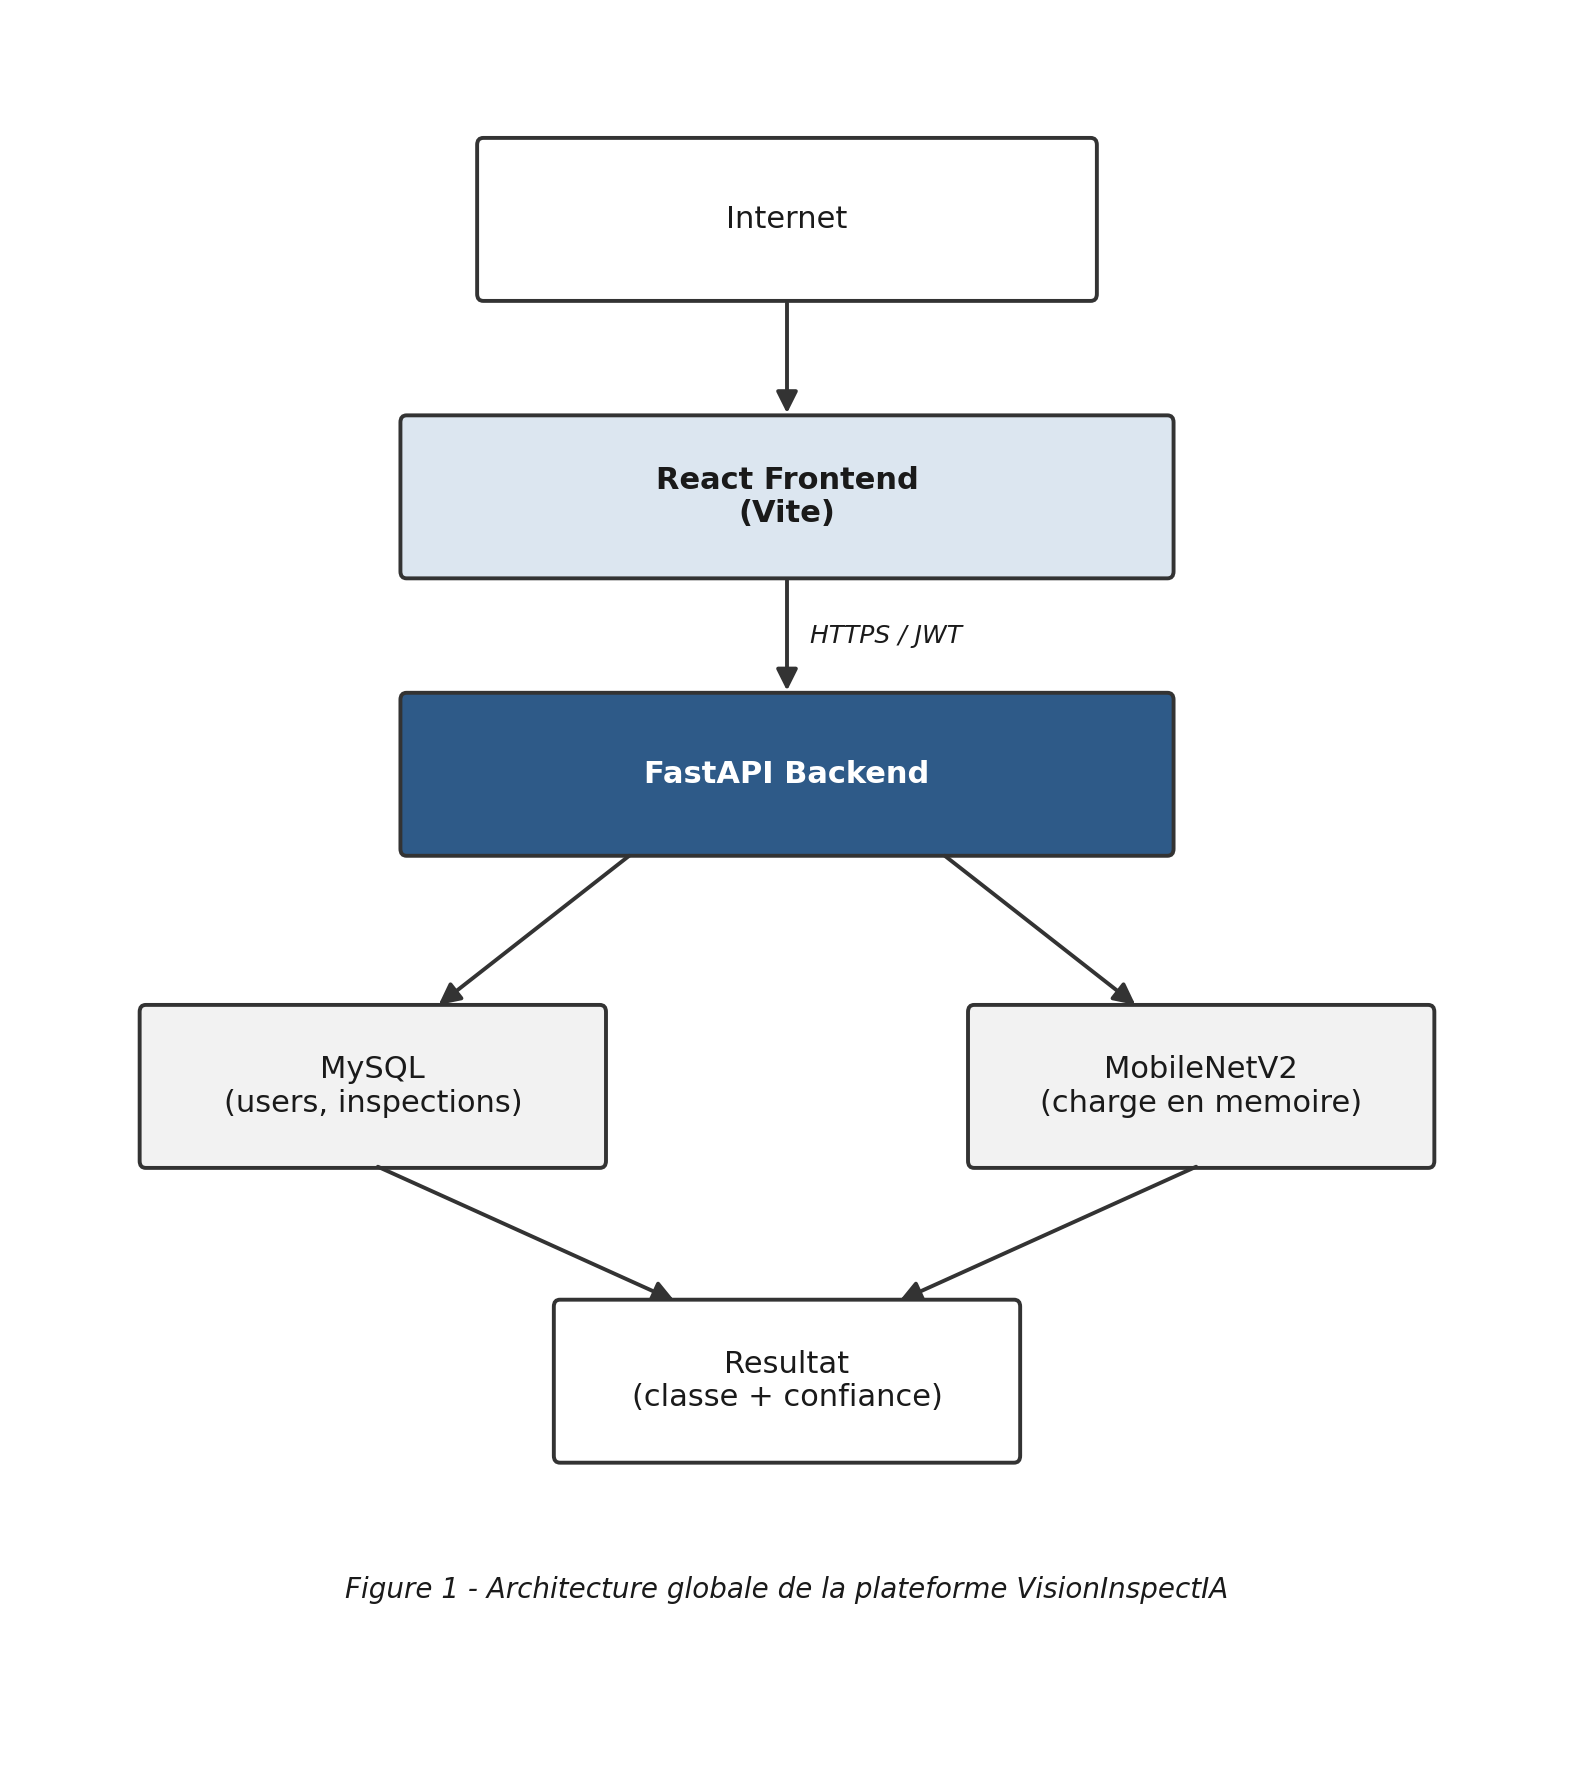
\includegraphics[width=0.6\textwidth]{figure_01_architecture_globale.png}
\caption{Architecture globale de la plateforme VisionInspectIA.}
\label{fig:architecture-globale}
\end{figure}

Comme pr\'esent\'e \`a la \Cref{fig:architecture-globale}, le frontend React communique en HTTPS/JWT avec le backend FastAPI, qui est le seul point d'entr\'ee vers MySQL (donn\'ees) et vers MobileNetV2 (IA, charg\'e en m\'emoire dans le m\^eme processus backend, et non dans un service s\'epar\'e).

\section{Frontend}

Application React (b\^atie avec Vite), organis\'ee en couches~: \texttt{api/} (appels HTTP centralis\'es), \texttt{context/}/\texttt{hooks/} (\'etat global~: authentification, th\`eme, notifications), \texttt{components/} (par fonctionnalit\'e), \texttt{pages/} (\'ecrans), \texttt{routes/} (protection des pages priv\'ees).

\section{Backend}

API FastAPI organis\'ee en couches strictes~: \texttt{api/} (routes HTTP uniquement), \texttt{services/} (toute la logique m\'etier), \texttt{models/} (tables SQLAlchemy), \texttt{schemas/} (validation Pydantic), \texttt{ml/} (chargement du mod\`ele et pr\'etraitement), \texttt{db/}, \texttt{core/}.

\section{IA}

Le mod\`ele MobileNetV2 est charg\'e une seule fois en m\'emoire au d\'emarrage du serveur (voir \Cref{ch:ia-prediction}) et interrog\'e \`a chaque requ\^ete de pr\'ediction, sans rechargement.

\section{Base de donn\'ees}

MySQL, acc\'ed\'ee via SQLAlchemy (ORM), d\'etaill\'ee au \Cref{ch:database}.

\section{Authentification}

Authentification par jeton JWT (voir \Cref{ch:backend}), avec hachage des mots de passe par bcrypt.

\section{Communication frontend/backend}

Communication exclusivement via une API REST en JSON (et \texttt{multipart/form-data} pour l'upload d'image), s\'ecuris\'ee par HTTPS en production et prot\'eg\'ee par une politique CORS restreinte \`a l'origine du frontend d\'eploy\'e (voir \Cref{ch:deploiement}).

\section{Gestion des fichiers}

Les images upload\'ees sont stock\'ees sur le syst\`eme de fichiers du serveur backend (\texttt{backend/uploads/}), servies statiquement, et r\'ef\'erenc\'ees en base par leur chemin relatif. Cette approche pr\'esente une limite en environnement cloud, discut\'ee au \Cref{ch:deploiement} et au \Cref{ch:discussion}.

\section{S\'ecurit\'e}

Isolation stricte des donn\'ees entre utilisateurs (chaque requ\^ete est filtr\'ee sur l'identifiant de l'utilisateur authentifi\'e), gestion explicite des codes d'erreur HTTP (401, 400, 404), variables sensibles (\texttt{SECRET\_KEY}, identifiants de base de donn\'ees) exclusivement g\'er\'ees via variables d'environnement, jamais versionn\'ees.

\chapter{Base de donn\'ees}
\label{ch:database}

\section{Choix de MySQL}

MySQL a \'et\'e retenu conform\'ement au cahier des charges, qui l'imposait explicitement comme syst\`eme de gestion de base de donn\'ees pour ce projet~\cite{mysql}.

\section{Mod\`ele de donn\'ees}

\begin{figure}[H]
\centering
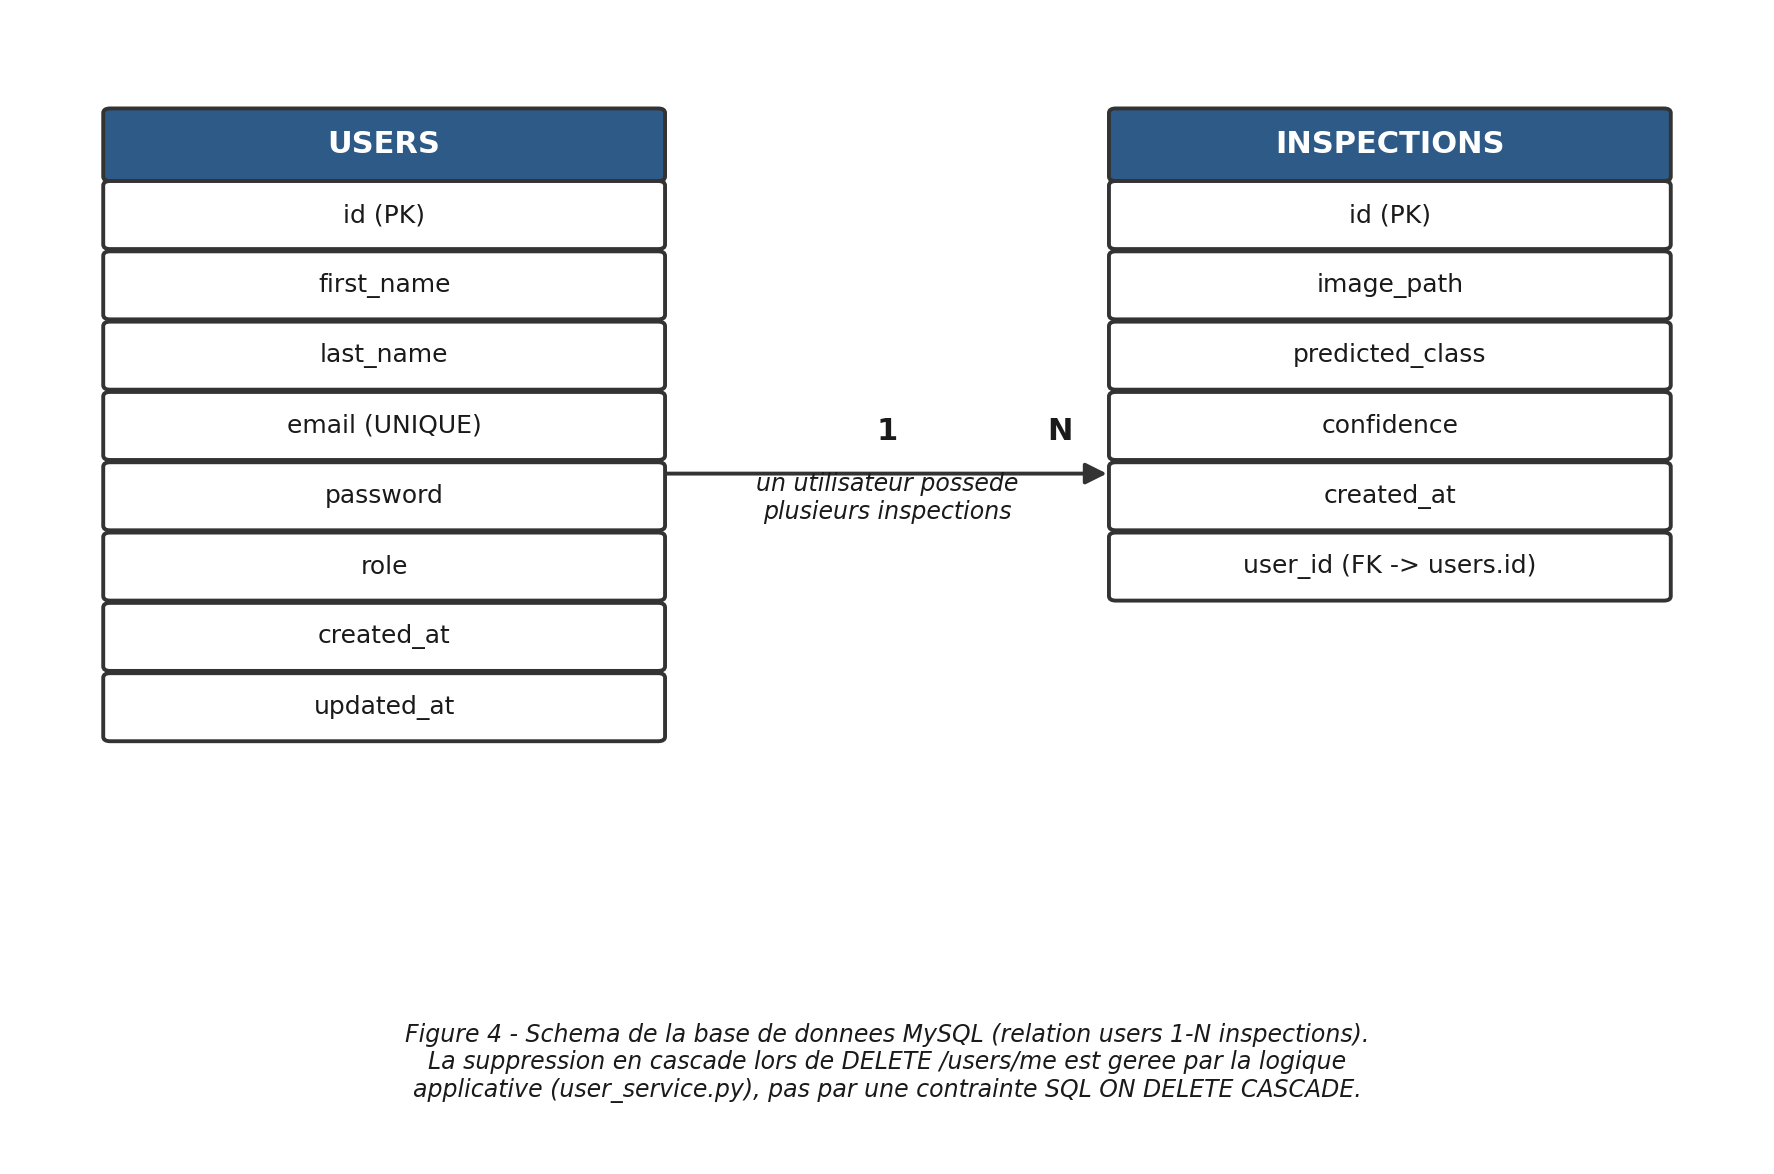
\includegraphics[width=0.85\textwidth]{figure_04_bdd_erd.png}
\caption{Sch\'ema de la base de donn\'ees MySQL (relation \texttt{users} 1--N \texttt{inspections}).}
\label{fig:erd}
\end{figure}

\begin{table}[H]
\centering
\caption{Table \texttt{users} (source~: \texttt{backend/app/models/user.py})}
\label{tab:table-users}
\begin{tabular}{lll}
\toprule
Champ & Type & Contrainte \\
\midrule
\texttt{id} & Integer & Cl\'e primaire \\
\texttt{first\_name} & String(100) & Non nul \\
\texttt{last\_name} & String(100) & Non nul \\
\texttt{email} & String(255) & Unique, index\'e, non nul \\
\texttt{password} & String(255) & Non nul (hash bcrypt) \\
\texttt{role} & String(50) & Non nul, d\'efaut \texttt{"user"} \\
\texttt{created\_at} & DateTime & Automatique \\
\texttt{updated\_at} & DateTime & Automatique \\
\bottomrule
\end{tabular}
\end{table}

\begin{table}[H]
\centering
\caption{Table \texttt{inspections} (source~: \texttt{backend/app/models/inspection.py})}
\label{tab:table-inspections}
\begin{tabular}{lll}
\toprule
Champ & Type & Contrainte \\
\midrule
\texttt{id} & Integer & Cl\'e primaire \\
\texttt{image\_path} & String(500) & Non nul \\
\texttt{predicted\_class} & String(100) & Non nul \\
\texttt{confidence} & Float & Non nul \\
\texttt{created\_at} & DateTime & Automatique \\
\texttt{user\_id} & Integer & Cl\'e \'etrang\`ere $\rightarrow$ \texttt{users.id}, non nul \\
\bottomrule
\end{tabular}
\end{table}

\textbf{Relation~:} \texttt{users}~(1) --- (N)~\texttt{inspections}.

\section{Contraintes}

Cl\'e \'etrang\`ere \texttt{inspections.user\_id} $\rightarrow$ \texttt{users.id}~; contrainte d'unicit\'e sur \texttt{users.email}.

\section{Isolation des utilisateurs}

Toute requ\^ete portant sur les inspections filtre syst\'ematiquement sur l'identifiant de l'utilisateur authentifi\'e (extrait du JWT), emp\^echant un utilisateur d'acc\'eder aux donn\'ees d'un autre (v\'erifi\'e en production, voir \Cref{ch:tests}).

\section{Gestion des inspections}

La suppression d'un compte utilisateur entra\^ine, au niveau de la logique applicative (\texttt{user\_service.py}), la suppression des inspections associ\'ees ainsi que des fichiers image correspondants sur le disque, avant la suppression de la ligne \texttt{users}.

\begin{noteflag}{Point important}
Il ne s'agit \textbf{pas} d'une cascade d\'eclar\'ee au niveau du sch\'ema SQL (\texttt{ON DELETE CASCADE}), mais d'une suppression orchestr\'ee par le code applicatif.
\end{noteflag}

\section{D\'eploiement de MySQL sur Railway}

En production, la base de donn\'ees est un service MySQL manag\'e par Railway (plugin officiel), accessible uniquement depuis le r\'eseau priv\'e du projet (non expos\'e publiquement). Les tables sont cr\'e\'ees automatiquement au d\'emarrage du backend via l'appel de la fonction \texttt{init\_db()} (voir \Cref{ch:deploiement}, correction apport\'ee pendant le d\'eploiement).

Alembic est configur\'e dans le projet (\texttt{backend/alembic/}) mais \textbf{aucune migration versionn\'ee n'a \'et\'e g\'en\'er\'ee} \`a ce jour --- le r\'epertoire \texttt{backend/alembic/versions/} ne contient qu'un fichier \texttt{.gitkeep}. Le sch\'ema est actuellement g\'er\'e exclusivement via \texttt{Base.metadata.create\_all()}, sans historique de migrations.

\chapter{Backend FastAPI}
\label{ch:backend}

\section{Pr\'esentation de FastAPI}

FastAPI a \'et\'e retenu, parmi les deux options propos\'ees par le cahier des charges (FastAPI ou Flask), pour sa validation de donn\'ees native via Pydantic, sa g\'en\'eration automatique de documentation interactive (Swagger/ReDoc), et son support natif de l'asynchrone~\cite{fastapi}.

\section{Architecture backend}

\begin{lstlisting}[language=, basicstyle=\ttfamily\small, frame=single]
app/
|-- core/       # Configuration, securite (hash, JWT)
|-- api/        # Routes HTTP uniquement
|-- db/         # Connexion et session SQLAlchemy
|-- models/     # Tables SQLAlchemy
|-- schemas/    # Validation Pydantic
|-- services/   # Toute la logique metier
|-- ml/         # Chargement du modele et pretraitement
`-- utils/      # Fonctions utilitaires (fichiers, PDF)
\end{lstlisting}

\section{Configuration}

La configuration (\texttt{app/core/config.py}) est centralis\'ee via \texttt{pydantic-settings}, permettant une surcharge compl\`ete par variables d'environnement (base de donn\'ees, JWT, CORS, port d'\'ecoute), sans valeur sensible cod\'ee en dur.

\section{Authentification JWT}

Un jeton JWT (algorithme HS256) est \'emis \`a la connexion et doit \^etre fourni via l'en-t\^ete \texttt{Authorization: Bearer <token>} pour toute route prot\'eg\'ee. Sa dur\'ee de validit\'e est configurable (\texttt{ACCESS\_TOKEN\_EXPIRE\_MINUTES}).

\section{Gestion des utilisateurs}

Inscription, connexion, consultation et modification du profil, changement de mot de passe, suppression de compte.

\section{Upload}

L'upload d'image se fait en \texttt{multipart/form-data}, avec validation du format et de la taille du fichier avant tout traitement (\texttt{backend/app/utils/file\_utils.py}).

\section{Pipeline de pr\'ediction}

D\'etaill\'e au \Cref{ch:ia-prediction}.

\section{Historique}

Liste, d\'etail et suppression des inspections, filtr\'ees sur l'utilisateur courant.

\section{Dashboard}

Statistiques agr\'eg\'ees calcul\'ees par requ\^ete SQL (\texttt{COUNT}, \texttt{SUM} conditionnel, \texttt{AVG}) sur MySQL, jamais pr\'e-calcul\'ees ni stock\'ees (\texttt{backend/app/services/dashboard\_service.py}).

\section{PDF}

G\'en\'eration de rapport PDF en m\'emoire (ReportLab), sans \'ecriture de fichier temporaire sur le disque (\texttt{backend/app/utils/pdf\_utils.py}).

\section{S\'ecurit\'e}

Voir \Cref{ch:architecture} et \Cref{ch:database}.

\section{API REST}

\begin{table}[H]
\centering
\small
\caption{Endpoints de l'API REST (source~: \texttt{backend/app/api/v1/router.py})}
\label{tab:endpoints}
\begin{tabular}{lll l}
\toprule
M\'ethode & Endpoint & Auth & Fonction \\
\midrule
POST & \texttt{/api/v1/auth/register} & Non & Cr\'eation de compte \\
POST & \texttt{/api/v1/auth/login} & Non & Connexion, \'emission du JWT \\
GET & \texttt{/api/v1/auth/me} & Oui & Profil de l'utilisateur courant \\
POST & \texttt{/api/v1/auth/logout} & Oui & D\'econnexion \\
PUT & \texttt{/api/v1/users/me} & Oui & Modification du profil \\
PUT & \texttt{/api/v1/users/me/password} & Oui & Changement de mot de passe \\
DELETE & \texttt{/api/v1/users/me} & Oui & Suppression du compte \\
POST & \texttt{/api/v1/predictions/predict} & Oui & Upload d'image + pr\'ediction \\
GET & \texttt{/api/v1/history} & Oui & Liste des inspections \\
GET & \texttt{/api/v1/history/\{id\}} & Oui & D\'etail d'une inspection \\
DELETE & \texttt{/api/v1/history/\{id\}} & Oui & Suppression d'une inspection \\
GET & \texttt{/api/v1/dashboard/statistics} & Oui & Statistiques agr\'eg\'ees \\
GET & \texttt{/api/v1/reports/\{inspection\_id\}} & Oui & G\'en\'eration du rapport PDF \\
\bottomrule
\end{tabular}
\end{table}

Chaque groupe de routes dispose \'egalement d'un endpoint \texttt{GET /health} sans logique m\'etier associ\'ee.

\chapter{Frontend React}
\label{ch:frontend}

\section{Choix de React}

React a \'et\'e retenu parmi les deux options propos\'ees par le cahier des charges (React ou Angular)~\cite{react}.

\section{Architecture frontend}

\begin{lstlisting}[language=, basicstyle=\ttfamily\small, frame=single]
src/
|-- api/          # Appels HTTP centralises
|-- components/   # Composants reutilisables, par fonctionnalite
|-- pages/        # Ecrans
|-- context/      # Etat global (Auth, Theme, Toast)
|-- hooks/        # Hooks personnalises
|-- routes/       # Routage et protection des pages privees
|-- layouts/      # Mise en page commune
`-- utils/        # Statistiques dashboard, export CSV
\end{lstlisting}

\section{Routing}

G\'er\'e par React Router (\texttt{src/routes/AppRoutes.jsx}), avec protection des pages priv\'ees (redirection vers \texttt{/login} en l'absence de session valide).

\section{AuthContext}

Contexte React centralisant l'\'etat d'authentification (token, utilisateur courant), consomm\'e par l'ensemble de l'application via un hook d\'edi\'e (\texttt{useAuth}).

\section{Axios}

Client HTTP centralis\'e (\texttt{src/api/axiosClient.js}), injectant automatiquement le JWT dans l'en-t\^ete \texttt{Authorization} de chaque requ\^ete, et g\'erant globalement l'expiration de session (redirection automatique en cas de r\'eponse 401).

\section{Login / Register}

Pages d\'edi\'ees, consommant respectivement \texttt{POST /auth/login} et \texttt{POST /auth/register}.

\section{Dashboard}

Page affichant les statistiques agr\'eg\'ees et les graphiques.

\section{Prediction}

Page d'upload et d'affichage du r\'esultat de pr\'ediction.

\section{History}

Page listant les inspections, avec recherche, filtres, tri et pagination.

\section{Profile}

Page de gestion du profil (\'edition, changement de mot de passe, suppression de compte).

\section{PDF et CSV}

T\'el\'echargement du rapport PDF depuis l'historique~; export CSV de l'historique, g\'en\'er\'e enti\`erement c\^ot\'e client.

\section{Notifications}

Centre de notifications (\texttt{ToastContext}).

\section{Dark mode}

Basculement de th\`eme clair/sombre, persist\'e dans le \texttt{localStorage} du navigateur (\texttt{ThemeContext}).

\section{Responsive design}

Interface con\c{c}ue pour s'adapter aux diff\'erentes tailles d'\'ecran (desktop, tablette, mobile).

\section{UX/UI --- limite importante}

\begin{noteflag}{Important}
L'environnement de d\'eveloppement utilis\'e pour ce projet ne disposait pas de navigateur graphique. Le rendu visuel effectif (mise en page, comportement du mode sombre, comportement responsive r\'eel) \textbf{n'a pas pu \^etre v\'erifi\'e visuellement} au cours du d\'eveloppement ni de la r\'edaction de ce rapport. Les fonctionnalit\'es correspondantes ont \'et\'e valid\'ees uniquement par revue du code source et par des tests fonctionnels au niveau de l'API (voir \Cref{ch:tests}). Aucune affirmation de type \guillemotleft~redesign moderne valid\'e visuellement~\guillemotright\ n'est donc formul\'ee dans ce rapport au-del\`a de ce qui a \'et\'e effectivement v\'erifi\'e.
\end{noteflag}

\section{Fonctionnalit\'es de la plateforme}

\begin{table}[H]
\centering
\small
\caption{Fonctionnalit\'es implement\'ees et leur statut de v\'erification}
\label{tab:fonctionnalites}
\begin{tabularx}{\textwidth}{lXX}
\toprule
Fonctionnalit\'e & Fonctionnement & R\'esultat \\
\midrule
Register & \texttt{POST /auth/register}, mot de passe hach\'e (bcrypt) & Compte cr\'e\'e, v\'erifi\'e fonctionnel en local et en production \\
Login & \texttt{POST /auth/login}, \'emission d'un JWT & JWT valide retourn\'e, v\'erifi\'e fonctionnel \\
Logout & \texttt{POST /auth/logout} & V\'erifi\'e fonctionnel \\
Dashboard & \texttt{GET /dashboard/statistics}, graphiques & Statistiques coh\'erentes avec les donn\'ees r\'eelles de MySQL \\
Prediction & Upload $\rightarrow$ \texttt{POST /predictions/predict} & Fonctionnel sur les 4~classes~; limite connue sur \texttt{broken\_small} \\
History & \texttt{GET /history}, recherche, filtres, tri, pagination & Fonctionnel \\
Inspection details & \texttt{GET /history/\{id\}}, modal de d\'etail & Fonctionnel, isolation entre utilisateurs v\'erifi\'ee \\
PDF & \texttt{GET /reports/\{inspection\_id\}}, g\'en\'er\'e en m\'emoire & Fonctionnel, y compris en d\'egrad\'e sans image \\
CSV & G\'en\'eration c\^ot\'e client (Blob) & Fonctionnel \\
Notifications & Centre de notifications (\texttt{ToastContext}) & Impl\'ement\'e~; v\'erification visuelle non r\'ealis\'ee \\
Dark mode & Bascule de th\`eme, persist\'ee en \texttt{localStorage} & Impl\'ement\'e~; v\'erification visuelle non r\'ealis\'ee \\
Profile & \texttt{PUT /users/me} & Test\'e en production, fonctionnel \\
Change password & \texttt{PUT /users/me/password} & Test\'e en production, fonctionnel \\
Delete account & \texttt{DELETE /users/me}, suppression en cascade & Test\'e en production, cascade v\'erifi\'ee \\
\bottomrule
\end{tabularx}
\end{table}

\chapter{Pipeline de pr\'ediction IA}
\label{ch:ia-prediction}

Le pipeline de pr\'ediction, identique en d\'eveloppement et en production, se d\'eroule comme suit (source~: \texttt{backend/app/services/prediction\_service.py})~:

\begin{figure}[H]
\centering
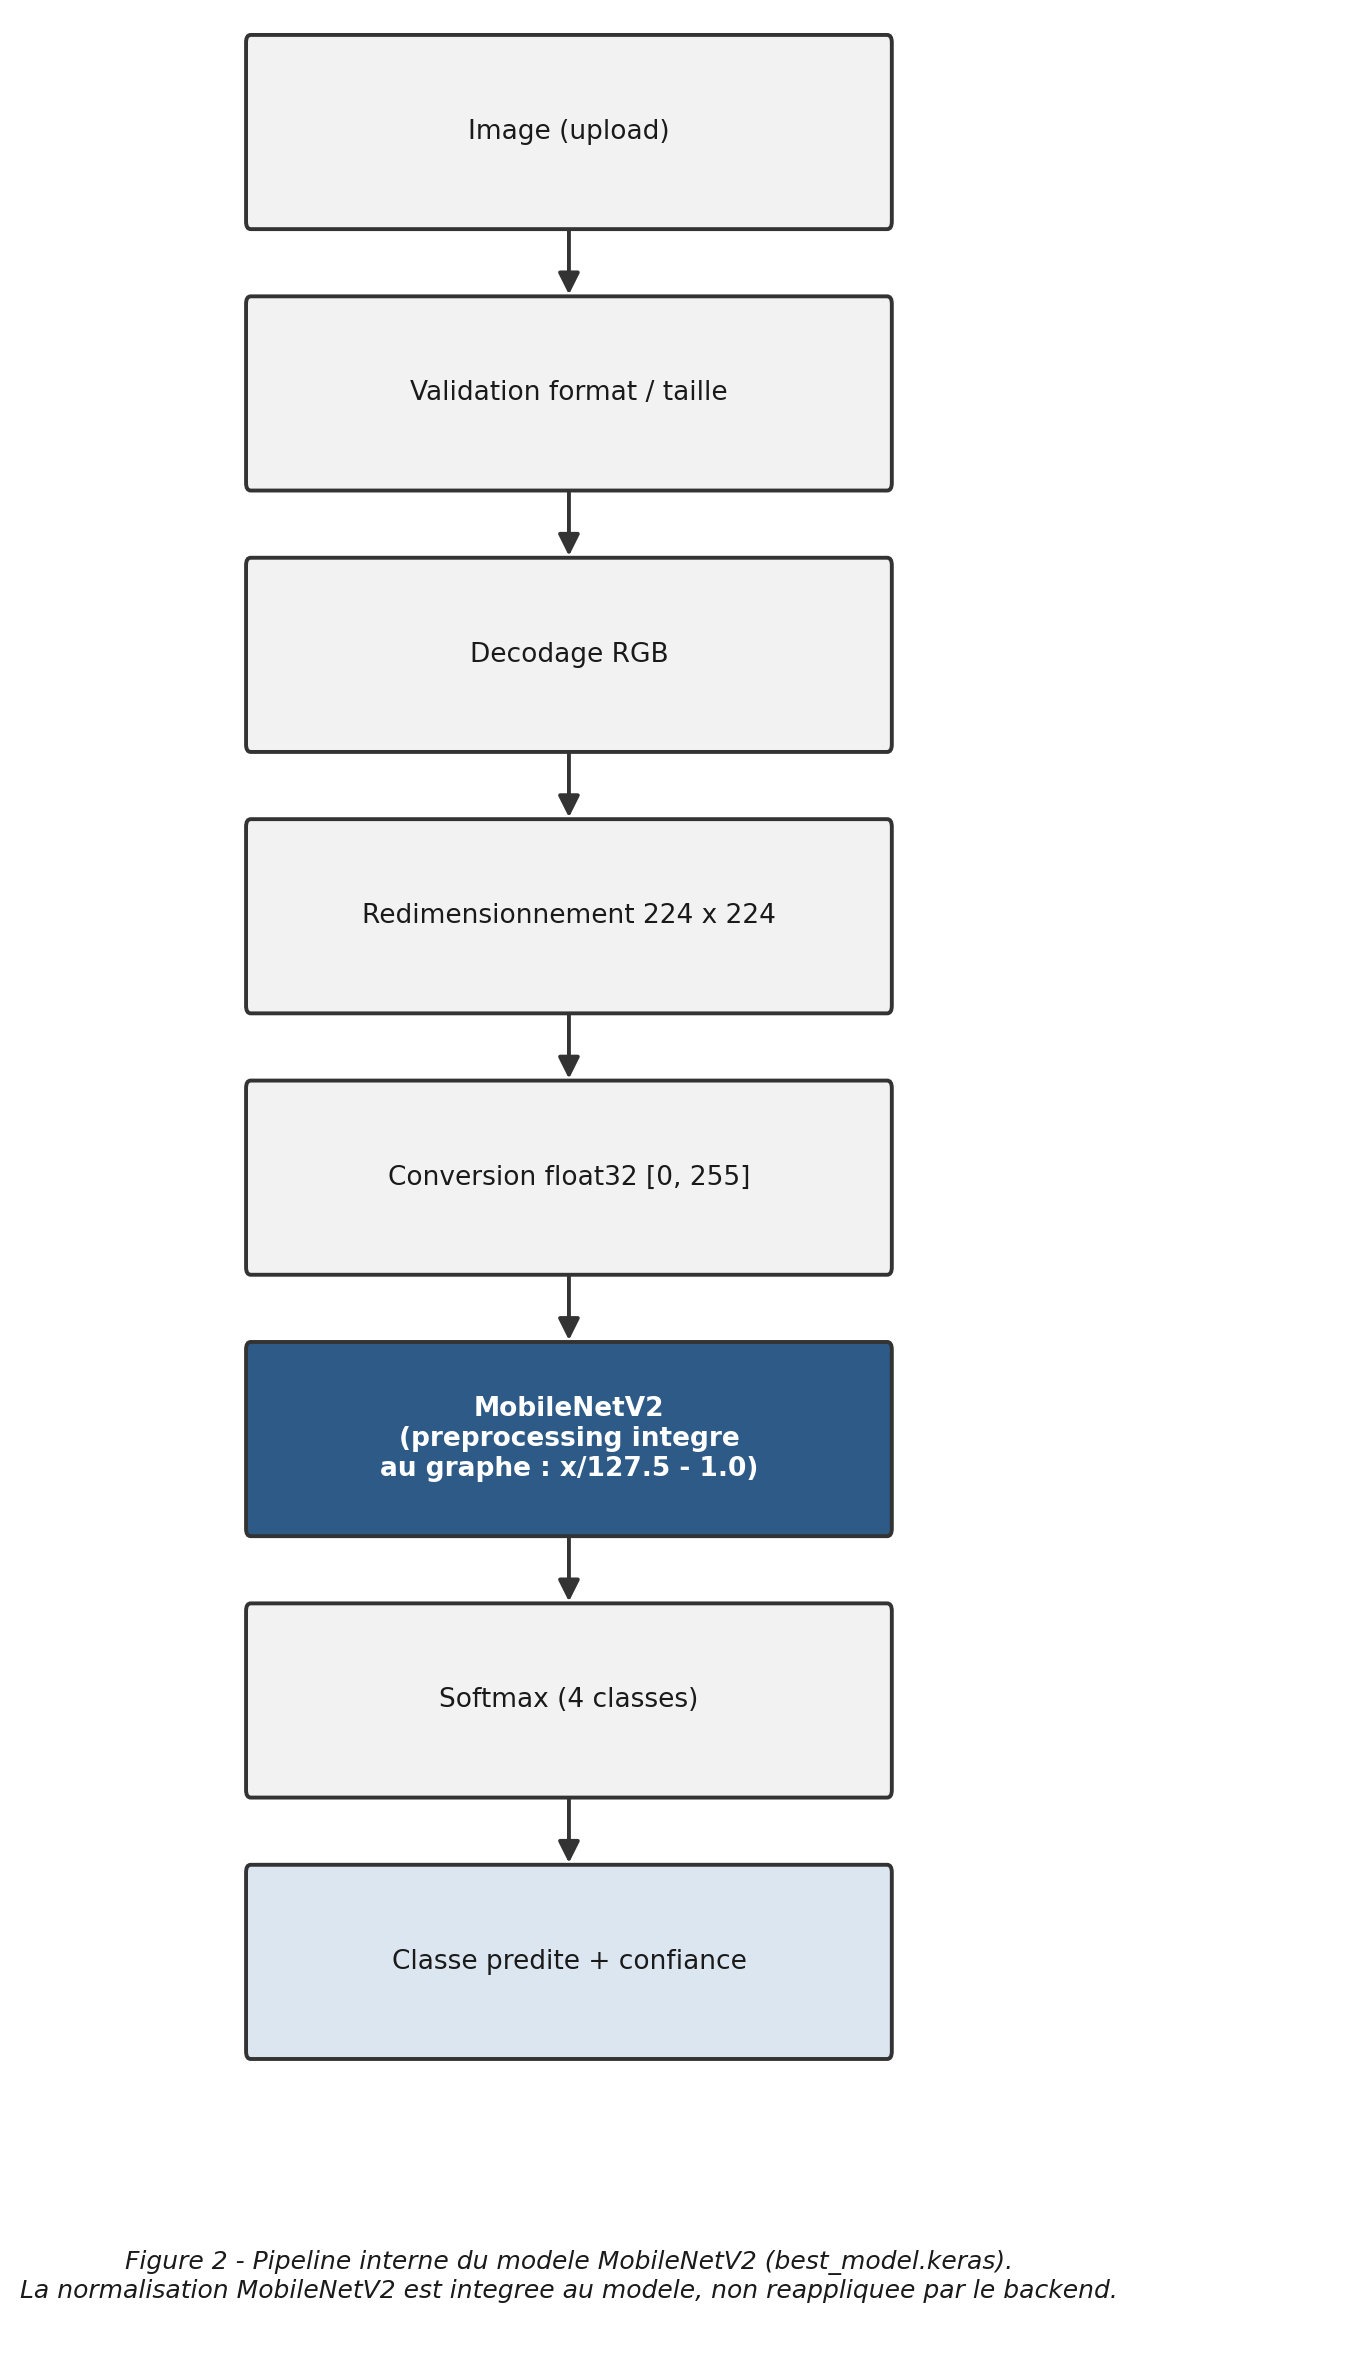
\includegraphics[width=0.5\textwidth]{figure_02_architecture_ia.png}
\caption{Pipeline interne du mod\`ele MobileNetV2 (\texttt{best\_model.keras}).}
\label{fig:pipeline-ia}
\end{figure}

\begin{figure}[H]
\centering
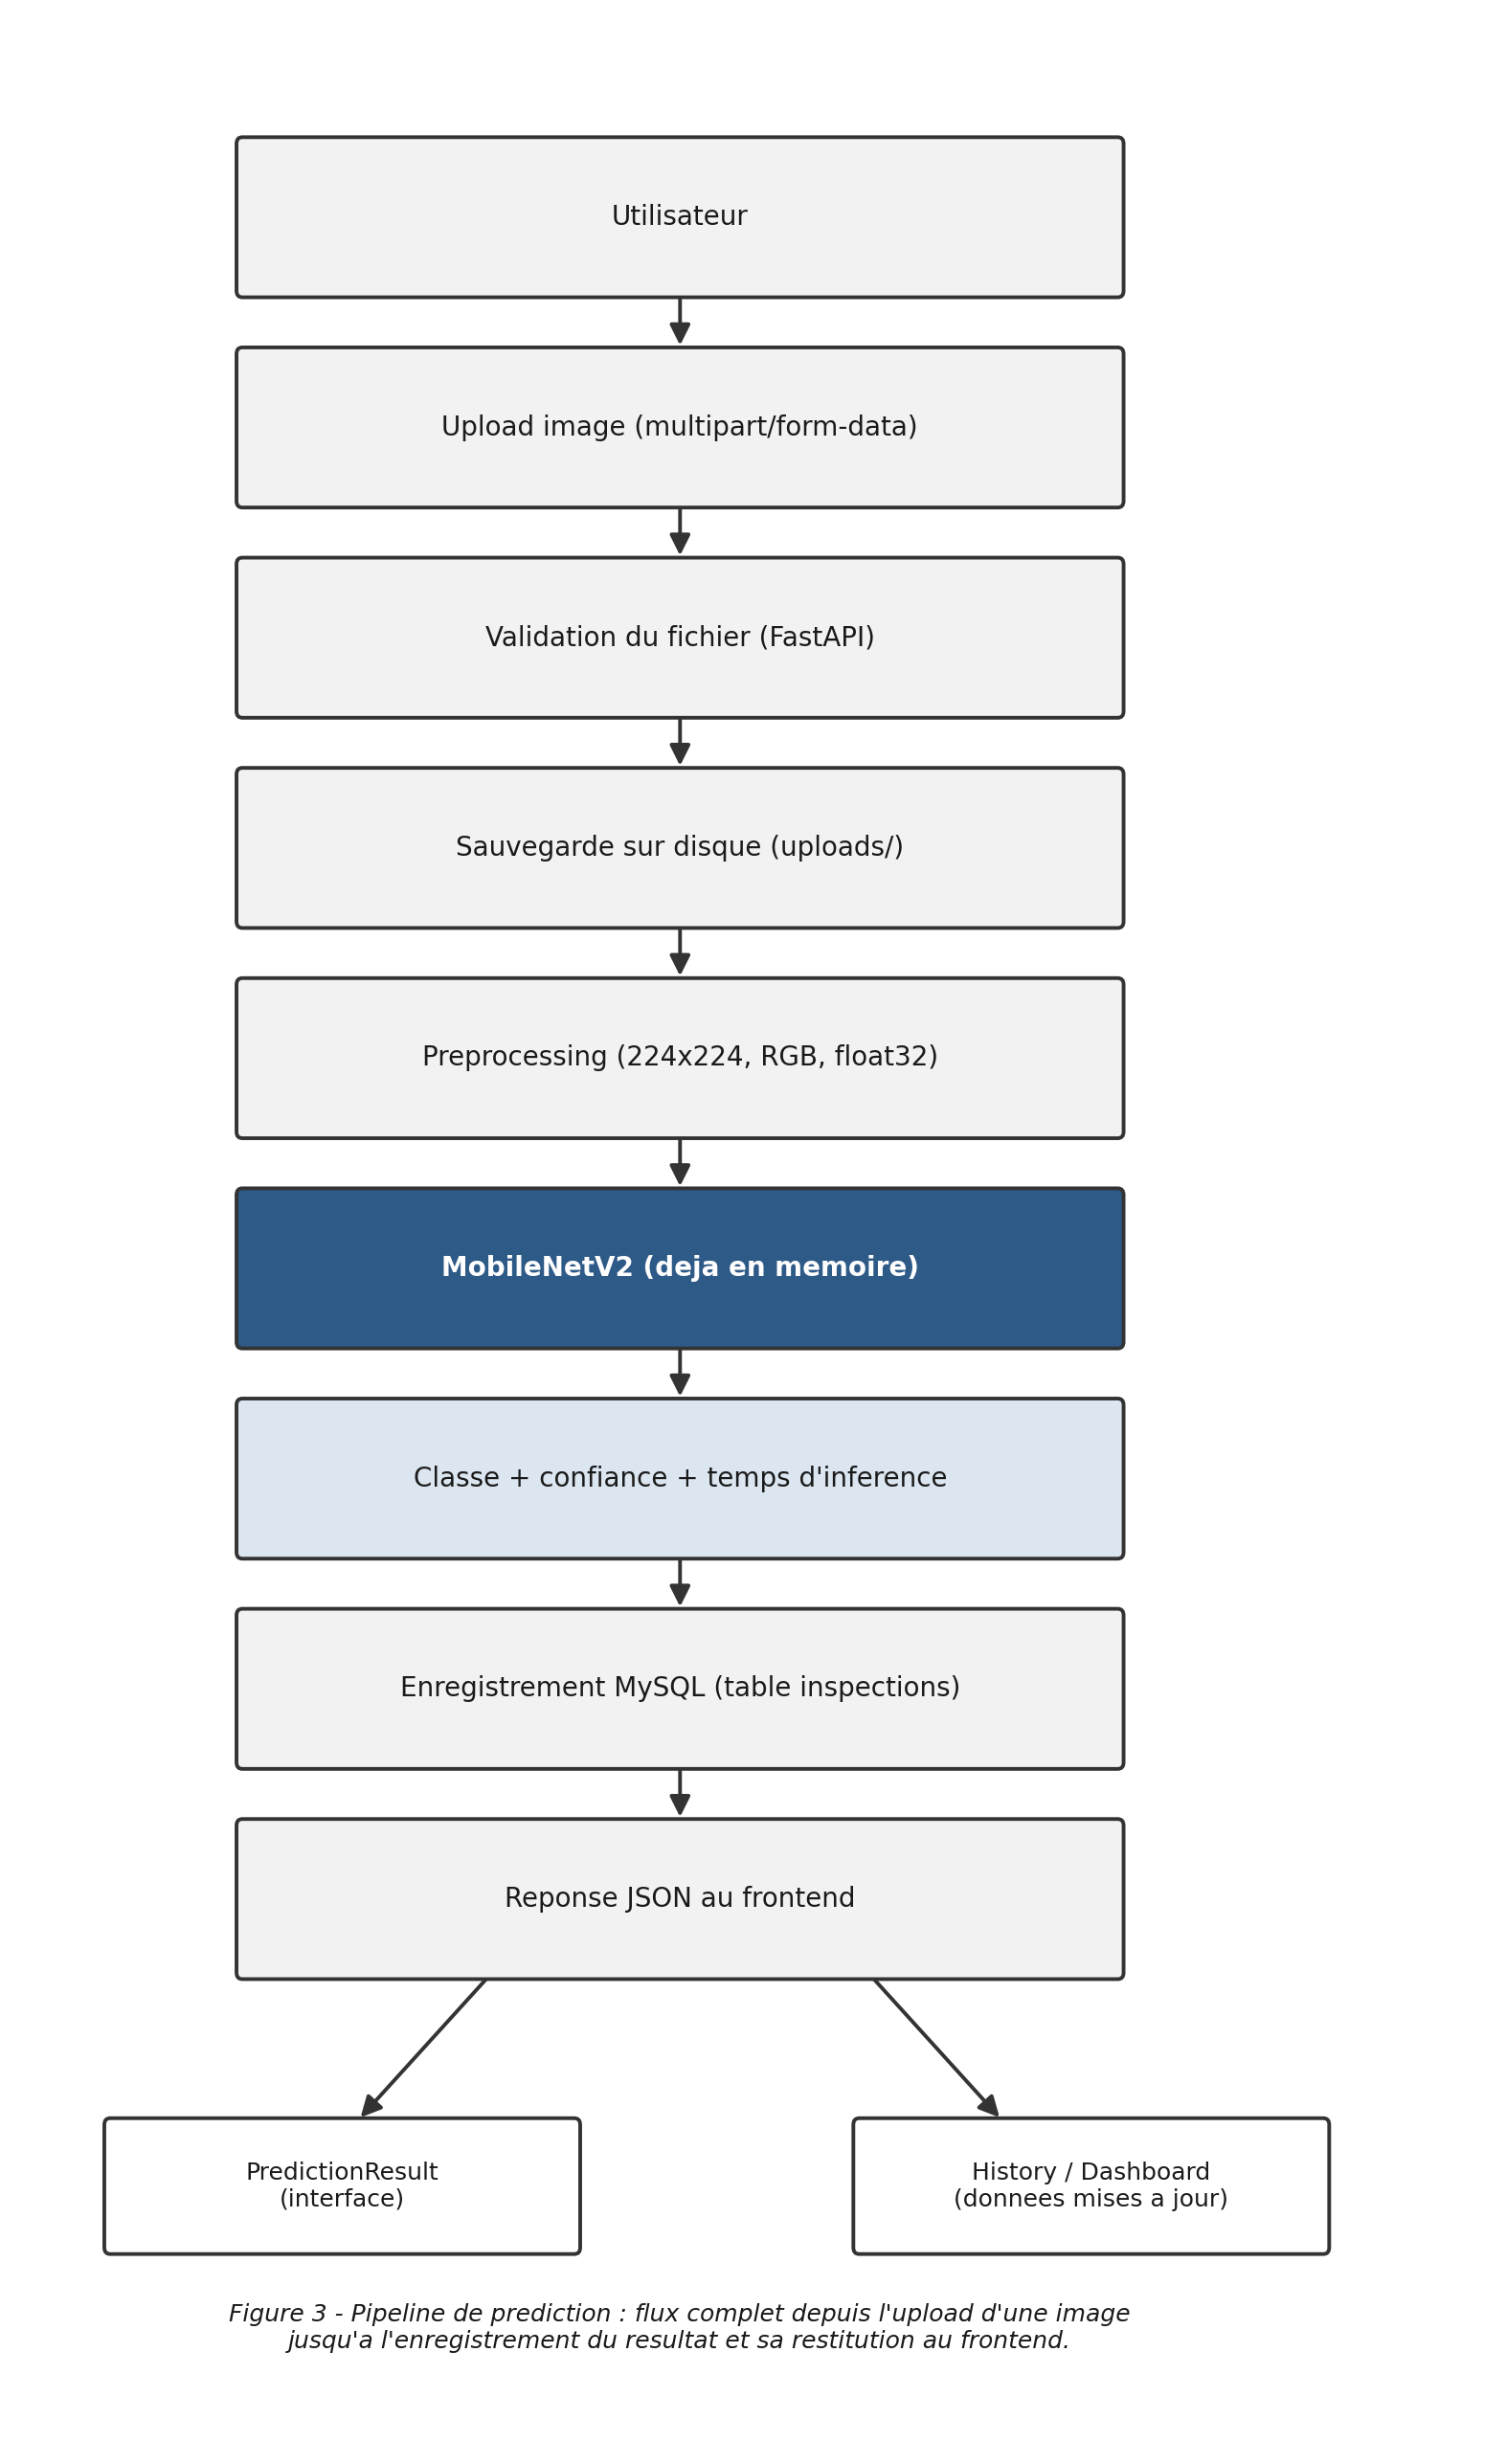
\includegraphics[width=0.62\textwidth]{figure_03_pipeline_prediction.png}
\caption{Pipeline de pr\'ediction~: flux applicatif complet depuis l'upload jusqu'\`a la r\'eponse.}
\label{fig:pipeline-prediction}
\end{figure}

Comme le montre la \Cref{fig:pipeline-prediction}, les \'etapes sont~:
\begin{enumerate}
  \item upload de l'image (multipart/form-data)~;
  \item validation du format et de la taille du fichier~;
  \item sauvegarde sur disque (\texttt{backend/uploads/})~;
  \item pr\'etraitement (224$\times$224, RGB, \texttt{float32})~;
  \item inf\'erence MobileNetV2 (mod\`ele d\'ej\`a en m\'emoire)~;
  \item calcul de la classe pr\'edite et du score de confiance (softmax)~;
  \item enregistrement de l'inspection en base MySQL~;
  \item r\'eponse JSON au frontend (classe, confiance, temps d'inf\'erence).
\end{enumerate}

\textbf{Chargement du mod\`ele.} Le fichier \texttt{best\_model.keras} est charg\'e une seule fois en m\'emoire au d\'emarrage du serveur (fonction \texttt{lifespan} de \texttt{backend/app/main.py}), via un singleton (\texttt{ModelLoader}). Il n'est jamais recharg\'e par la suite, chaque requ\^ete de pr\'ediction r\'eutilisant l'instance d\'ej\`a en m\'emoire.

\textbf{Temps d'inf\'erence.} Le temps d'inf\'erence pure (appel \texttt{model.predict()} uniquement, mod\`ele d\'ej\`a charg\'e) est mesur\'e \`a chaque pr\'ediction via \texttt{time.perf\_counter()} et retourn\'e au frontend dans la r\'eponse JSON (champ \texttt{inference\_time\_ms}), sans \^etre persist\'e en base de donn\'ees. La valeur mesur\'ee lors du benchmark (\Cref{ch:modelisation}) est d'environ 9~ms~; les temps mesur\'es en production, incluant le trajet HTTP complet, sont pr\'esent\'es au \Cref{ch:deploiement}.

\begin{noteflag}{Point de conception important}
Le preprocessing MobileNetV2 (\texttt{x/127,5 -- 1,0}) est int\'egr\'e directement au graphe du mod\`ele sauvegard\'e (couche \texttt{MobileNetPreprocess}). Le backend ne r\'eapplique donc \textbf{pas} une seconde normalisation lors du pr\'etraitement --- ce point a \'et\'e v\'erifi\'e explicitement pour \'eviter de fausser les pr\'edictions (voir \Cref{ch:dataset}).
\end{noteflag}

\chapter{Tests et validation}
\label{ch:tests}

\section{Tests backend}

D\'emarrage du serveur, disponibilit\'e de la documentation interactive (\texttt{/docs}, \texttt{/redoc}), connexion \`a MySQL.

\section{Tests frontend}

Build de production (\texttt{npm run build})~: 2505~modules transform\'es, 0~erreur, v\'erifi\'e \`a plusieurs reprises au cours du projet.

\section{Tests API}

Ensemble des endpoints list\'es au \Cref{tab:endpoints}, test\'es par des requ\^etes HTTP r\'eelles (et non simul\'ees).

\section{Tests IA}

Pr\'ediction test\'ee sur une image de chacune des quatre classes, en local puis en production.

\section{Tests s\'ecurit\'e}

Acc\`es sans JWT, JWT invalide, tentative d'acc\`es aux donn\'ees d'un autre utilisateur --- tous test\'es et confirm\'es bloqu\'es (codes 401/404 appropri\'es), y compris en production.

\section{Tests base de donn\'ees}

V\'erification du sch\'ema, des contraintes (cl\'e \'etrang\`ere, unicit\'e de l'email), et de la coh\'erence entre les fichiers du dossier \texttt{uploads/} et les lignes correspondantes en base.

\section{Tests PDF}

G\'en\'eration v\'erifi\'ee sur des inspections r\'eelles, y compris en d\'egrad\'e lorsque le fichier image n'est plus disponible.

\section{Tests CSV}

G\'en\'eration v\'erifi\'ee sur des donn\'ees r\'eelles d'historique.

\section{Tests end-to-end}

Sc\'enario complet ex\'ecut\'e en local puis en production~: inscription $\rightarrow$ connexion $\rightarrow$ upload $\rightarrow$ pr\'ediction $\rightarrow$ historique $\rightarrow$ tableau de bord $\rightarrow$ PDF $\rightarrow$ modification du profil $\rightarrow$ d\'econnexion.

\section{Tests en production}

\begin{table}[H]
\centering
\small
\caption{Tests en production (requ\^etes HTTP r\'eelles contre les URLs publiques de d\'eploiement)}
\label{tab:tests-production}
\begin{tabularx}{\textwidth}{lXl}
\toprule
Fonctionnalit\'e & Test & R\'esultat \\
\midrule
Frontend accessible & \texttt{GET /} et routes SPA & \okmark\ 200 sur toutes les routes \\
Backend accessible & \texttt{GET /} & \okmark\ 200 \\
Swagger / ReDoc & \texttt{GET /docs}, \texttt{GET /redoc} & \okmark\ 200 / 200 \\
Register & \texttt{POST /auth/register} & \okmark\ 201 \\
Login & bon et mauvais mot de passe & \okmark\ 200 / 401 \\
Prediction --- \texttt{good} & Upload r\'eel & \okmark\ correct, confiance 99,4\,\% \\
Prediction --- \texttt{broken\_large} & Upload r\'eel & \okmark\ correct, confiance 99,8\,\% \\
Prediction --- \texttt{broken\_small} & Upload r\'eel & \warnmark\ \textbf{incorrect}, pr\'edit \texttt{broken\_large} (80,5\,\%) \\
Prediction --- \texttt{contamination} & Upload r\'eel & \okmark\ correct, confiance 99,3\,\% \\
History & \texttt{GET /history} & \okmark\ coh\'erent apr\`es red\'eploiement \\
Dashboard & \texttt{GET /dashboard/statistics} & \okmark\ coh\'erent avec les inspections r\'eelles \\
PDF & \texttt{GET /reports/\{id\}} & \okmark\ 200, m\^eme si image absente \\
Profile & \texttt{PUT /users/me} & \okmark\ modifi\'e et confirm\'e \\
Change password & \texttt{PUT /users/me/password} & \okmark\ ancien rejet\'e, nouveau accept\'e \\
Delete account & \texttt{DELETE /users/me} & \okmark\ token r\'evoqu\'e, email r\'eutilisable \\
Logout & \texttt{POST /auth/logout} & \okmark\ 200 \\
Isolation entre utilisateurs & acc\`es \`a une ressource d'un autre utilisateur & \okmark\ 404 \\
Sans JWT / JWT invalide & \texttt{GET /history} & \okmark\ 401 / 401 \\
Fichier invalide & upload \texttt{.zip} & \okmark\ 400, message explicite \\
CORS & requ\^ete r\'eelle depuis le domaine du frontend & \okmark\ origine exacte, pas de wildcard \\
\bottomrule
\end{tabularx}
\end{table}

\begin{noteflag}{Sur \texttt{broken\_small}}
Ce r\'esultat n'est pas cach\'e~: il est conforme \`a la limite d\'ej\`a identifi\'ee lors du benchmark (\Cref{ch:modelisation}) et discut\'ee au \Cref{ch:discussion}.
\end{noteflag}

\chapter{D\'eploiement}
\label{ch:deploiement}

\section{Pourquoi Railway}

Parmi les trois plateformes propos\'ees par le cahier des charges (Render, Railway, Hugging Face Spaces), Railway~\cite{railway} a \'et\'e retenue apr\`es comparaison~: c'est la seule \`a proposer une base de donn\'ees MySQL manag\'ee nativement (Render ne propose pas de MySQL manag\'e, seulement PostgreSQL/Redis~; Hugging Face Spaces n'est pas con\c{c}u pour une application full-stack avec authentification et base de donn\'ees relationnelle). Railway permet ainsi d'h\'eberger backend, frontend et base de donn\'ees au sein d'un unique projet.

\section{Architecture de production}

\begin{figure}[H]
\centering
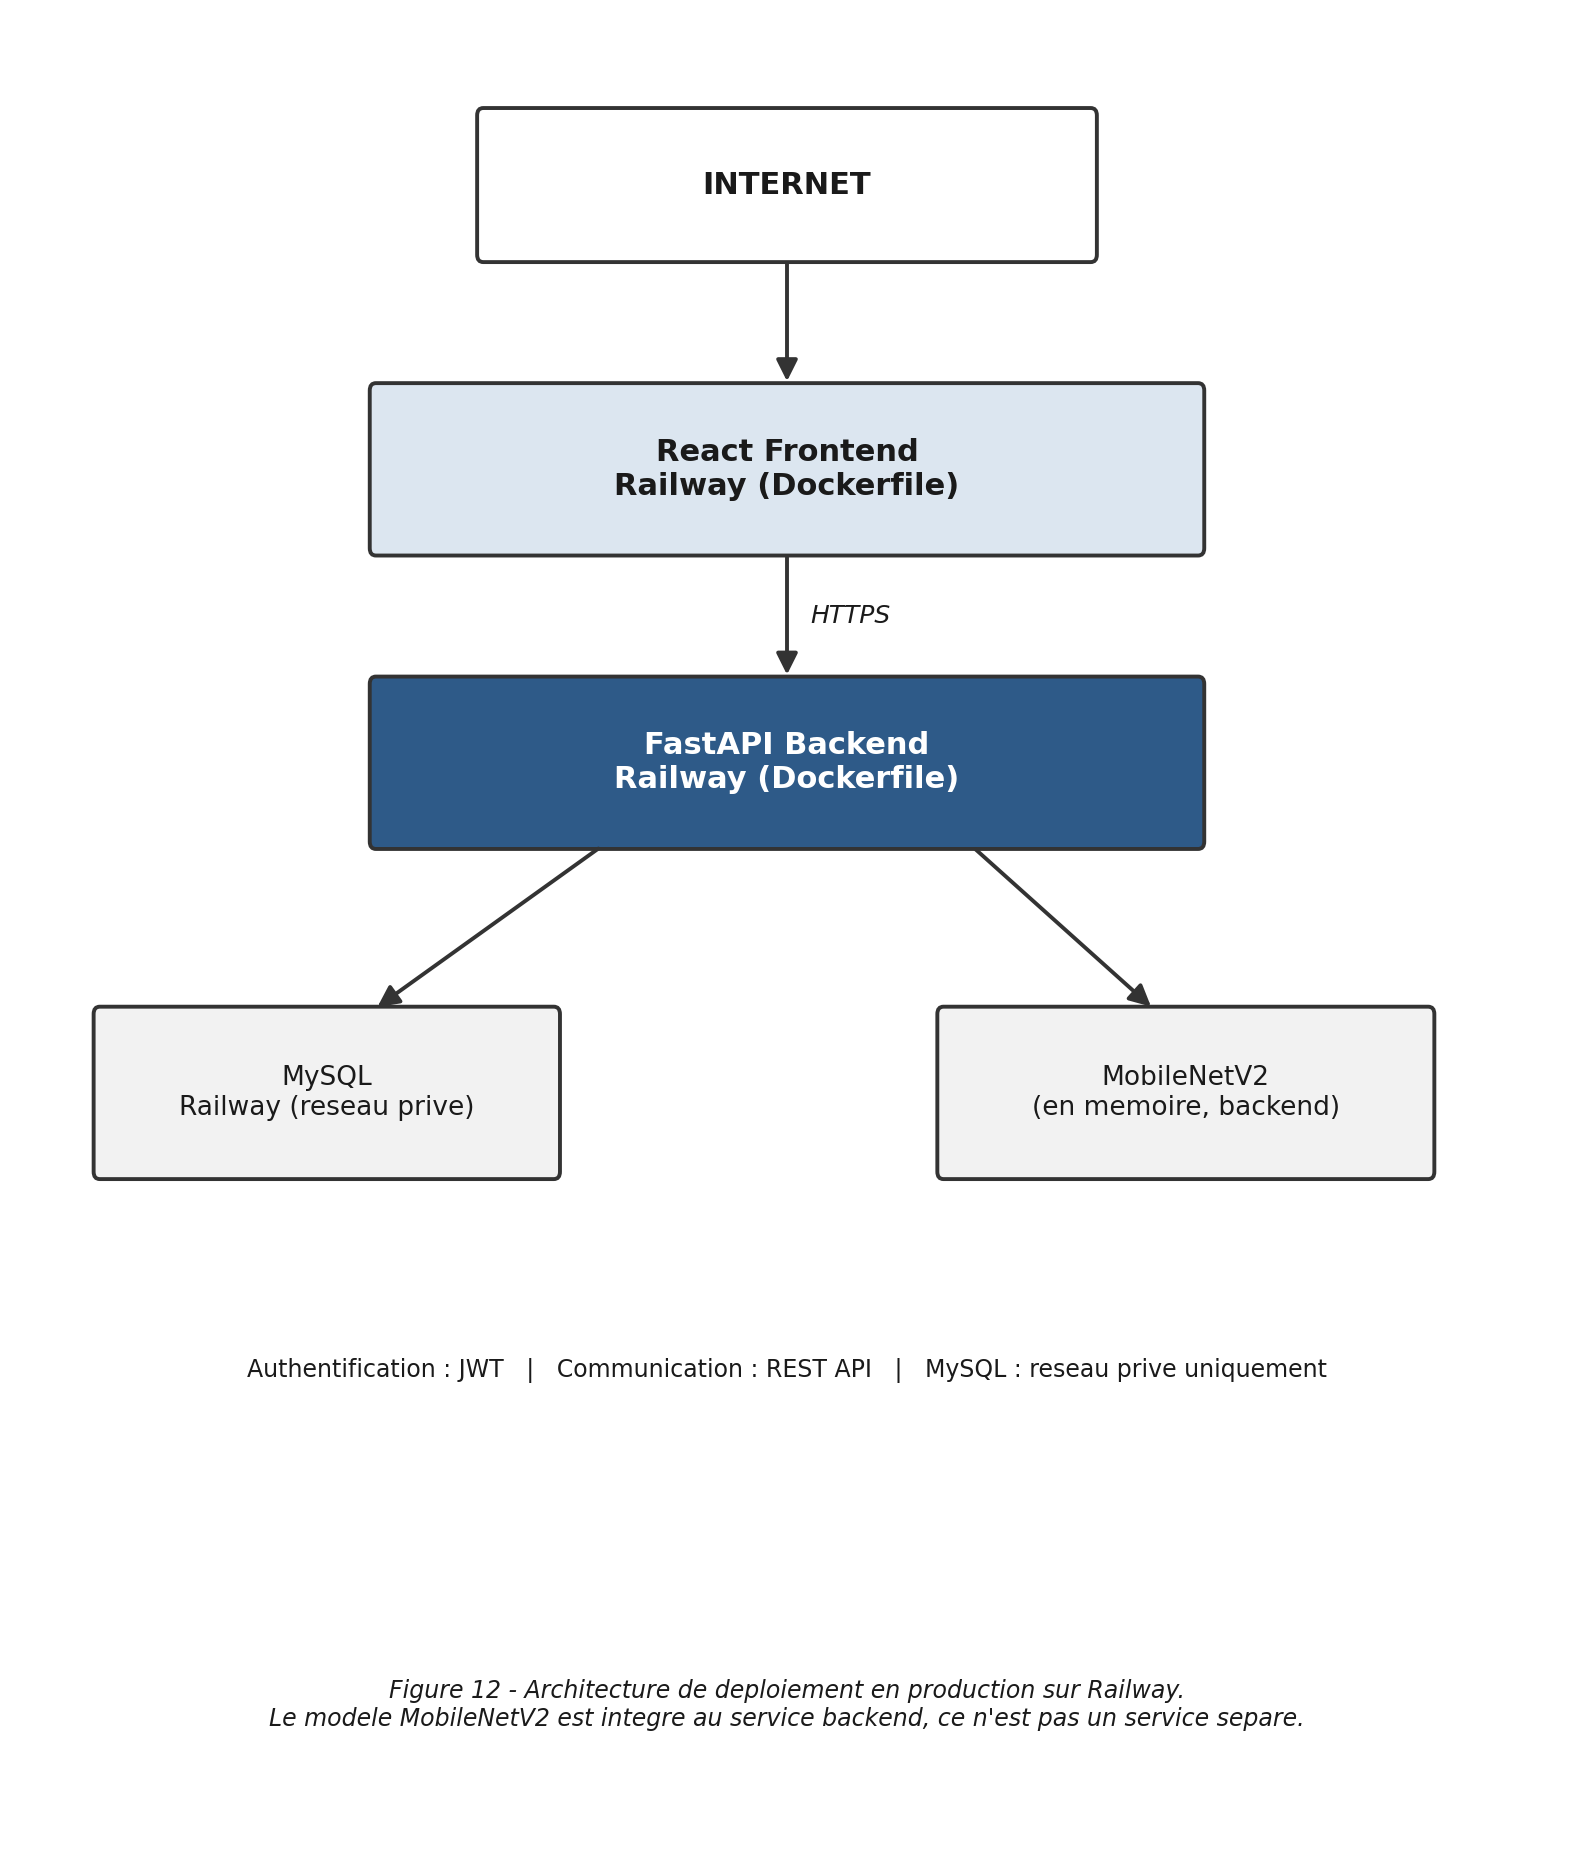
\includegraphics[width=0.55\textwidth]{figure_12_deploiement_railway.png}
\caption{Architecture de d\'eploiement en production sur Railway.}
\label{fig:deploiement-railway}
\end{figure}

\section{Docker}

Chaque service (backend, frontend) est d\'eploy\'e via un \texttt{Dockerfile} explicite (\texttt{backend/Dockerfile}, \texttt{frontend/Dockerfile}). Ce choix a \'et\'e fait apr\`es l'\'echec du builder automatique par d\'efaut de Railway (Railpack) sur la structure en monorepo du projet (voir \Cref{sec:problemes-deploiement}).

\section{Backend}

Service Railway distinct, \texttt{Root Directory = backend/}, construit \`a partir d'un \texttt{Dockerfile} (image \texttt{python:3.13-slim}, installation des d\'ependances via \texttt{pip}, lancement par \texttt{uvicorn}).

\section{Frontend}

Service Railway distinct, \texttt{Root Directory = frontend/}, construction en deux \'etapes (build Vite avec \texttt{VITE\_API\_URL} inject\'e comme argument de build Docker, puis service statique via le paquet \texttt{serve}).

\section{MySQL}

Base de donn\'ees provisionn\'ee via le plugin officiel MySQL de Railway, accessible uniquement en r\'eseau priv\'e au sein du projet.

\section{Variables d'environnement}

Les variables suivantes sont d\'efinies au niveau de chaque service Railway, jamais versionn\'ees dans le d\'ep\^ot Git~: \texttt{DATABASE\_HOST}, \texttt{DATABASE\_PORT}, \texttt{DATABASE\_USER}, \texttt{DATABASE\_PASSWORD}, \texttt{DATABASE\_NAME} (backend), \texttt{SECRET\_KEY}, \texttt{ALGORITHM}, \texttt{ACCESS\_TOKEN\_EXPIRE\_MINUTES}, \texttt{DEBUG}, \texttt{CORS\_ORIGINS} (backend), \texttt{VITE\_API\_URL} (frontend, en tant qu'argument de build).

\begin{noteflag}{S\'ecurit\'e}
Aucune valeur r\'eelle de ces variables n'est reproduite dans ce rapport ni dans le d\'ep\^ot (\texttt{backend/.env.example} ne contient que des placeholders).
\end{noteflag}

\section{MobileNetV2 en production}

Le backend embarque sa propre copie du mod\`ele (\texttt{backend/app/ml/model\_files/best\_model.keras}), rendant son d\'eploiement ind\'ependant du dossier \texttt{ai/}. L'identit\'e de cette copie avec le mod\`ele original a \'et\'e v\'erifi\'ee par comparaison d'empreinte SHA-256~: aucune modification des poids n'a \'et\'e introduite. Les journaux du service en production confirment le chargement effectif du mod\`ele au d\'emarrage (message \texttt{MobileNetV2 loaded successfully}).

\section{URLs}
\label{sec:urls}

\begin{itemize}
  \item \textbf{Frontend~:} \href{https://frontend-production-bcff.up.railway.app}{frontend-production-bcff.up.railway.app}
  \item \textbf{Backend~:} \href{https://visioninspectia-production.up.railway.app}{visioninspectia-production.up.railway.app}
  \item \textbf{Swagger~:} \href{https://visioninspectia-production.up.railway.app/docs}{visioninspectia-production.up.railway.app/docs}
  \item \textbf{ReDoc~:} \href{https://visioninspectia-production.up.railway.app/redoc}{visioninspectia-production.up.railway.app/redoc}
\end{itemize}

\section{Tests en production}

D\'etaill\'es au \Cref{ch:tests} (\Cref{tab:tests-production}).

\section{Performances}

Mesures r\'eellement observ\'ees en production (et non des estimations)~:
\begin{itemize}
  \item \textbf{Cold start} (premier appel apr\`es d\'emarrage, incluant le \emph{warm-up} TensorFlow)~: environ \textbf{1,9 \`a 2,3~secondes}.
  \item \textbf{Inf\'erence \`a chaud} (appels suivants, temps HTTP complet incluant upload, validation, pr\'etraitement, inf\'erence et \'ecriture en base)~: environ \textbf{170 \`a 210~ms}.
\end{itemize}

Ces deux valeurs sont \`a distinguer du temps d'inf\'erence pure mesur\'e lors du benchmark ($\approx$9~ms, \Cref{ch:modelisation}), qui ne couvre que l'appel au mod\`ele sur une image d\'ej\`a pr\'etrait\'ee, mod\`ele d\'ej\`a charg\'e.

\section{Probl\`emes rencontr\'es}
\label{sec:problemes-deploiement}

Le d\'eploiement a n\'ecessit\'e plusieurs it\'erations correctives, document\'ees ici pour leur valeur p\'edagogique~:

\begin{enumerate}
  \item \textbf{\'Echec de d\'etection par Railpack}~: le builder par d\'efaut de Railway ne parvenait pas \`a d\'etecter l'application depuis la racine du d\'ep\^ot (structure en monorepo).
  \item \textbf{D\'ependance du backend au dossier \texttt{ai/}}~: le chargement du mod\`ele r\'ef\'eren\c{c}ait initialement \texttt{ai/saved\_models/...} comme dossier fr\`ere de \texttt{backend/}, incompatible avec un d\'eploiement restreint \`a \texttt{backend/} seul.
  \item \textbf{\'Echec de d\'etection de la commande de d\'emarrage} par Railpack, y compris avec la commande d\'efinie c\^ot\'e service.
  \item \textbf{Erreur d'ordonnancement des couches de build} avec un fichier de configuration Railpack personnalis\'e.
  \item \textbf{Absence d'expansion de la variable \texttt{\$PORT}} lors du d\'emarrage du conteneur.
  \item \textbf{Configuration fig\'ee lors d'un red\'eploiement}~: la commande \texttt{redeploy} de Railway rejouait une configuration captur\'ee au moment du build pr\'ec\'edent.
  \item \textbf{Absence d'appel \`a \texttt{init\_db()}} au d\'emarrage, entra\^inant une erreur \guillemotleft~table inexistante~\guillemotright\ sur une base neuve.
  \item \textbf{Stockage non persistant} des images upload\'ees entre red\'eploiements (syst\`eme de fichiers \'eph\'em\`ere du conteneur).
\end{enumerate}

\section{Solutions appliqu\'ees}

\begin{itemize}
  \item \textbf{Points 1--2}~: le backend a \'et\'e rendu autonome par la duplication v\'erifi\'ee (empreinte SHA-256 identique) du fichier mod\`ele et de la couche de pr\'etraitement personnalis\'ee directement dans \texttt{backend/app/ml/}.
  \item \textbf{Points 3--5}~: abandon du builder automatique au profit d'un \textbf{Dockerfile explicite} par service.
  \item \textbf{Point 6}~: d\'eclenchement d'un nouveau commit Git (plut\^ot qu'un simple \texttt{redeploy}) pour forcer la prise en compte de la configuration \`a jour.
  \item \textbf{Point 7}~: ajout de l'appel \`a \texttt{init\_db()} dans la fonction \texttt{lifespan()} de \texttt{backend/app/main.py} --- modification idempotente, sans impact sur l'environnement de d\'eveloppement local existant.
  \item \textbf{Point 8}~: document\'ee explicitement comme limitation connue plut\^ot que trait\'ee par l'ajout d'une solution de stockage persistant, jug\'ee hors du p\'erim\`etre raisonnable pour une d\'emonstration de stage.
\end{itemize}

\chapter{R\'esultats, discussion, limitations et perspectives}
\label{ch:discussion}

\section{R\'esultats IA}

Voir \Cref{tab:benchmark} et \Cref{tab:classification-report} (\Cref{ch:modelisation}).

\section{Benchmark}

Le benchmark met en \'evidence l'apport d\'eterminant du transfer learning par rapport \`a un entra\^inement from scratch dans ce contexte de donn\'ees limit\'ees.

\section{Analyse par classe}

Les classes \texttt{good} et \texttt{broken\_large} sont d\'etect\'ees avec un rappel parfait par MobileNetV2 sur le jeu de test. Les classes \texttt{broken\_small} et \texttt{contamination} pr\'esentent un rappel plus faible (0,5 et 0,525 respectivement), traduisant une difficult\'e de discrimination plus importante pour ces d\'efauts.

\subsection*{Le cas \texttt{broken\_small}}

Cette classe constitue la principale limite de performance identifi\'ee dans ce projet, confirm\'ee \`a la fois sur le jeu de test et lors des tests en production (\Cref{ch:tests}, o\`u l'unique test r\'ealis\'e sur cette classe a \'et\'e mal class\'e). La cause la plus probable, au regard des donn\'ees disponibles, est le faible nombre d'images sources r\'eelles pour cette classe (22~images brutes au total, r\'eparties entre validation et test), rendant la distinction avec \texttt{broken\_large} difficile \`a apprendre de fa\c{c}on robuste.

\subsection*{Domain shift}

Aucune \'evaluation formelle de la robustesse du mod\`ele \`a un changement de domaine (images hors MVTec~AD) n'a \'et\'e r\'ealis\'ee dans ce projet. Ce point reste une perspective (voir \Cref{sec:perspectives}).

\section{R\'esultats applicatifs et production}

L'ensemble des fonctionnalit\'es list\'ees au cahier des charges a \'et\'e impl\'ement\'e et test\'e fonctionnellement (\Cref{ch:frontend}, \Cref{ch:tests}). L'application d\'eploy\'ee a \'et\'e test\'ee de bout en bout avec des requ\^etes r\'eelles contre les URLs publiques, confirmant son fonctionnement effectif au-del\`a de l'environnement de d\'eveloppement local.

\section{Discussion}

Il convient de distinguer clairement deux niveaux de performance \'evalu\'es dans ce projet~:
\begin{itemize}
  \item \textbf{La performance sur le jeu de test du dataset MVTec~AD}, qui reste, pour les classes \texttt{good}, \texttt{broken\_large} et \texttt{contamination}, \`a un niveau satisfaisant compte tenu du volume de donn\'ees disponible, mais qui repose sur un jeu de test partiellement constitu\'e d'images dupliqu\'ees \`a partir d'un faible nombre de sources uniques, ce qui limite la port\'ee statistique de ces chiffres.
  \item \textbf{La capacit\'e de g\'en\'eralisation au monde r\'eel}, c'est-\`a-dire \`a des photographies de bouteilles prises dans des conditions diff\'erentes de celles du dataset MVTec~AD (\'eclairage, arri\`ere-plan, appareil photo, cha\^ine de production r\'eelle), qui \textbf{n'a pas \'et\'e \'evalu\'ee} dans ce projet. Les tests r\'ealis\'es, y compris en production, utilisent exclusivement des images issues du m\^eme dataset que celui utilis\'e pour l'entra\^inement. Aucune affirmation de performance en conditions industrielles r\'eelles ne peut donc \^etre formul\'ee \`a partir des r\'esultats obtenus.
\end{itemize}

\section{Limitations}

\begin{table}[H]
\centering
\small
\caption{Limitations identifi\'ees}
\label{tab:limitations}
\begin{tabularx}{\textwidth}{lX}
\toprule
Limitation & Description \\
\midrule
Dataset limit\'e & Le dataset MVTec~AD (\emph{bottle}) ne compte que 292~images r\'eelles, avec seulement 20 \`a 22~images par classe de d\'efaut. \\
Difficult\'e sur \texttt{broken\_small} & Rappel de 0,5 sur le jeu de test, confirm\'e par un test en production~; confusion r\'ecurrente avec \texttt{broken\_large}. \\
Domain shift & La capacit\'e de g\'en\'eralisation \`a des images hors du dataset MVTec~AD n'a pas \'et\'e \'evalu\'ee. \\
Manque de photos terrain & Aucune photographie prise dans des conditions industrielles r\'eelles n'a \'et\'e utilis\'ee pour l'\'evaluation. \\
Stockage \texttt{uploads/} non persistant sur Railway & Le syst\`eme de fichiers du conteneur backend est \'eph\'em\`ere~; une image upload\'ee est perdue au red\'eploiement suivant (confirm\'e par test). Les donn\'ees en base ne sont pas affect\'ees. \\
Cold start TensorFlow & Premier appel apr\`es d\'emarrage sensiblement plus lent ($\approx$2~s) que les appels suivants. \\
Limites du tier Railway & Le projet est h\'eberg\'e sur l'offre gratuite/d'essai de Railway, sans garantie de disponibilit\'e prolong\'ee. \\
Absence de v\'erification visuelle & Le rendu effectif de l'interface (mode sombre, responsive) n'a pas pu \^etre v\'erifi\'e dans un navigateur r\'eel. \\
Alembic non exploit\'e & Alembic est configur\'e mais aucune migration versionn\'ee n'a \'et\'e g\'en\'er\'ee. \\
\bottomrule
\end{tabularx}
\end{table}

\section{Perspectives}
\label{sec:perspectives}

Les pistes suivantes sont pr\'esent\'ees comme des travaux futurs envisageables, \textbf{non impl\'ement\'es} dans la version actuelle du projet~:
\begin{itemize}
  \item enrichissement du dataset avec des photographies r\'eelles suppl\'ementaires, notamment pour la classe \texttt{broken\_small}~;
  \item collecte d'images en conditions industrielles r\'eelles, pour \'evaluer et am\'eliorer la robustesse au domain shift~;
  \item techniques d'augmentation plus avanc\'ees (ex. augmentation cibl\'ee sur les classes les plus faibles)~;
  \item mise en place d'un m\'ecanisme de d\'etection \emph{out-of-distribution} (rejet des images ne correspondant \`a aucune classe connue)~;
  \item migration vers un stockage cloud persistant (type S3) pour les images upload\'ees~;
  \item optimisation du mod\`ele pour un d\'eploiement plus l\'eger (par exemple conversion TensorFlow~Lite)~;
  \item mise en place de migrations Alembic versionn\'ees~;
  \item am\'elioration du pipeline de d\'eploiement (automatisation CI/CD, environnement de staging).
\end{itemize}

\chapter{Conclusion g\'en\'erale}
\label{ch:conclusion}

Ce stage a permis de mener un projet complet, de la pr\'eparation d'un dataset d'images industrielles jusqu'au d\'eploiement d'une application web fonctionnelle sur une infrastructure cloud r\'eelle, en couvrant les quatre phases d\'efinies par le cahier des charges TechSkillHub.

Sur le plan de l'intelligence artificielle, quatre architectures de classification d'images ont \'et\'e entra\^in\'ees et compar\'ees dans des conditions exp\'erimentales rigoureusement identiques. Cette comparaison a mis en \'evidence l'apport d\'eterminant du transfer learning face \`a un entra\^inement from scratch dans un contexte de donn\'ees limit\'ees, et a conduit \`a la s\'election de MobileNetV2, retenu non pas comme le mod\`ele le plus performant dans l'absolu, mais comme le meilleur compromis entre performance, taille et rapidit\'e d'inf\'erence pour une int\'egration dans une application web.

Sur le plan applicatif, une plateforme compl\`ete a \'et\'e d\'evelopp\'ee~: une API REST FastAPI structur\'ee en couches, une base de donn\'ees MySQL, et une interface React couvrant l'ensemble des fonctionnalit\'es attendues (authentification, pr\'ediction, historique, tableau de bord, export PDF/CSV, gestion du profil).

Sur le plan du d\'eploiement, l'application a \'et\'e r\'eellement mise en ligne sur Railway et test\'ee de bout en bout par des requ\^etes effectives contre les URLs publiques, d\'emarche qui a permis d'identifier et de corriger plusieurs probl\`emes concrets propres \`a un environnement de production (d\'ependances de build, gestion du port, initialisation de la base de donn\'ees), document\'es dans ce rapport \`a titre d'apprentissage technique.

Ce travail pr\'esente des limites clairement identifi\'ees~: une performance de d\'etection in\'egale selon les classes de d\'efaut (notamment sur \texttt{broken\_small}), une \'evaluation de g\'en\'eralisation au monde r\'eel non r\'ealis\'ee, et une contrainte de stockage propre \`a l'environnement de d\'eploiement choisi. Ces limites ne remettent pas en cause la validit\'e de la d\'emarche mise en \oe uvre, mais d\'elimitent pr\'ecis\'ement le p\'erim\`etre dans lequel les r\'esultats obtenus peuvent \^etre interpr\'et\'es.

Ce stage a permis de mettre en pratique, sur un cas d'usage industriel concret, l'ensemble d'une cha\^ine de traitement en intelligence artificielle appliqu\'ee~: de la donn\'ee brute \`a l'application d\'eploy\'ee, en passant par l'exp\'erimentation contr\^ol\'ee et l'\'evaluation critique des r\'esultats.


% ============================================================
% BIBLIOGRAPHIE
% ============================================================
\bibliographystyle{plain}
\bibliography{bibliography}
\addcontentsline{toc}{chapter}{Bibliographie}

% ============================================================
% ANNEXES
% ============================================================
\appendix
\chapter{Architecture globale}
\label{annex:architecture}

Voir \Cref{ch:architecture} et \Cref{fig:architecture-globale}.

\begin{figure}[H]
\centering
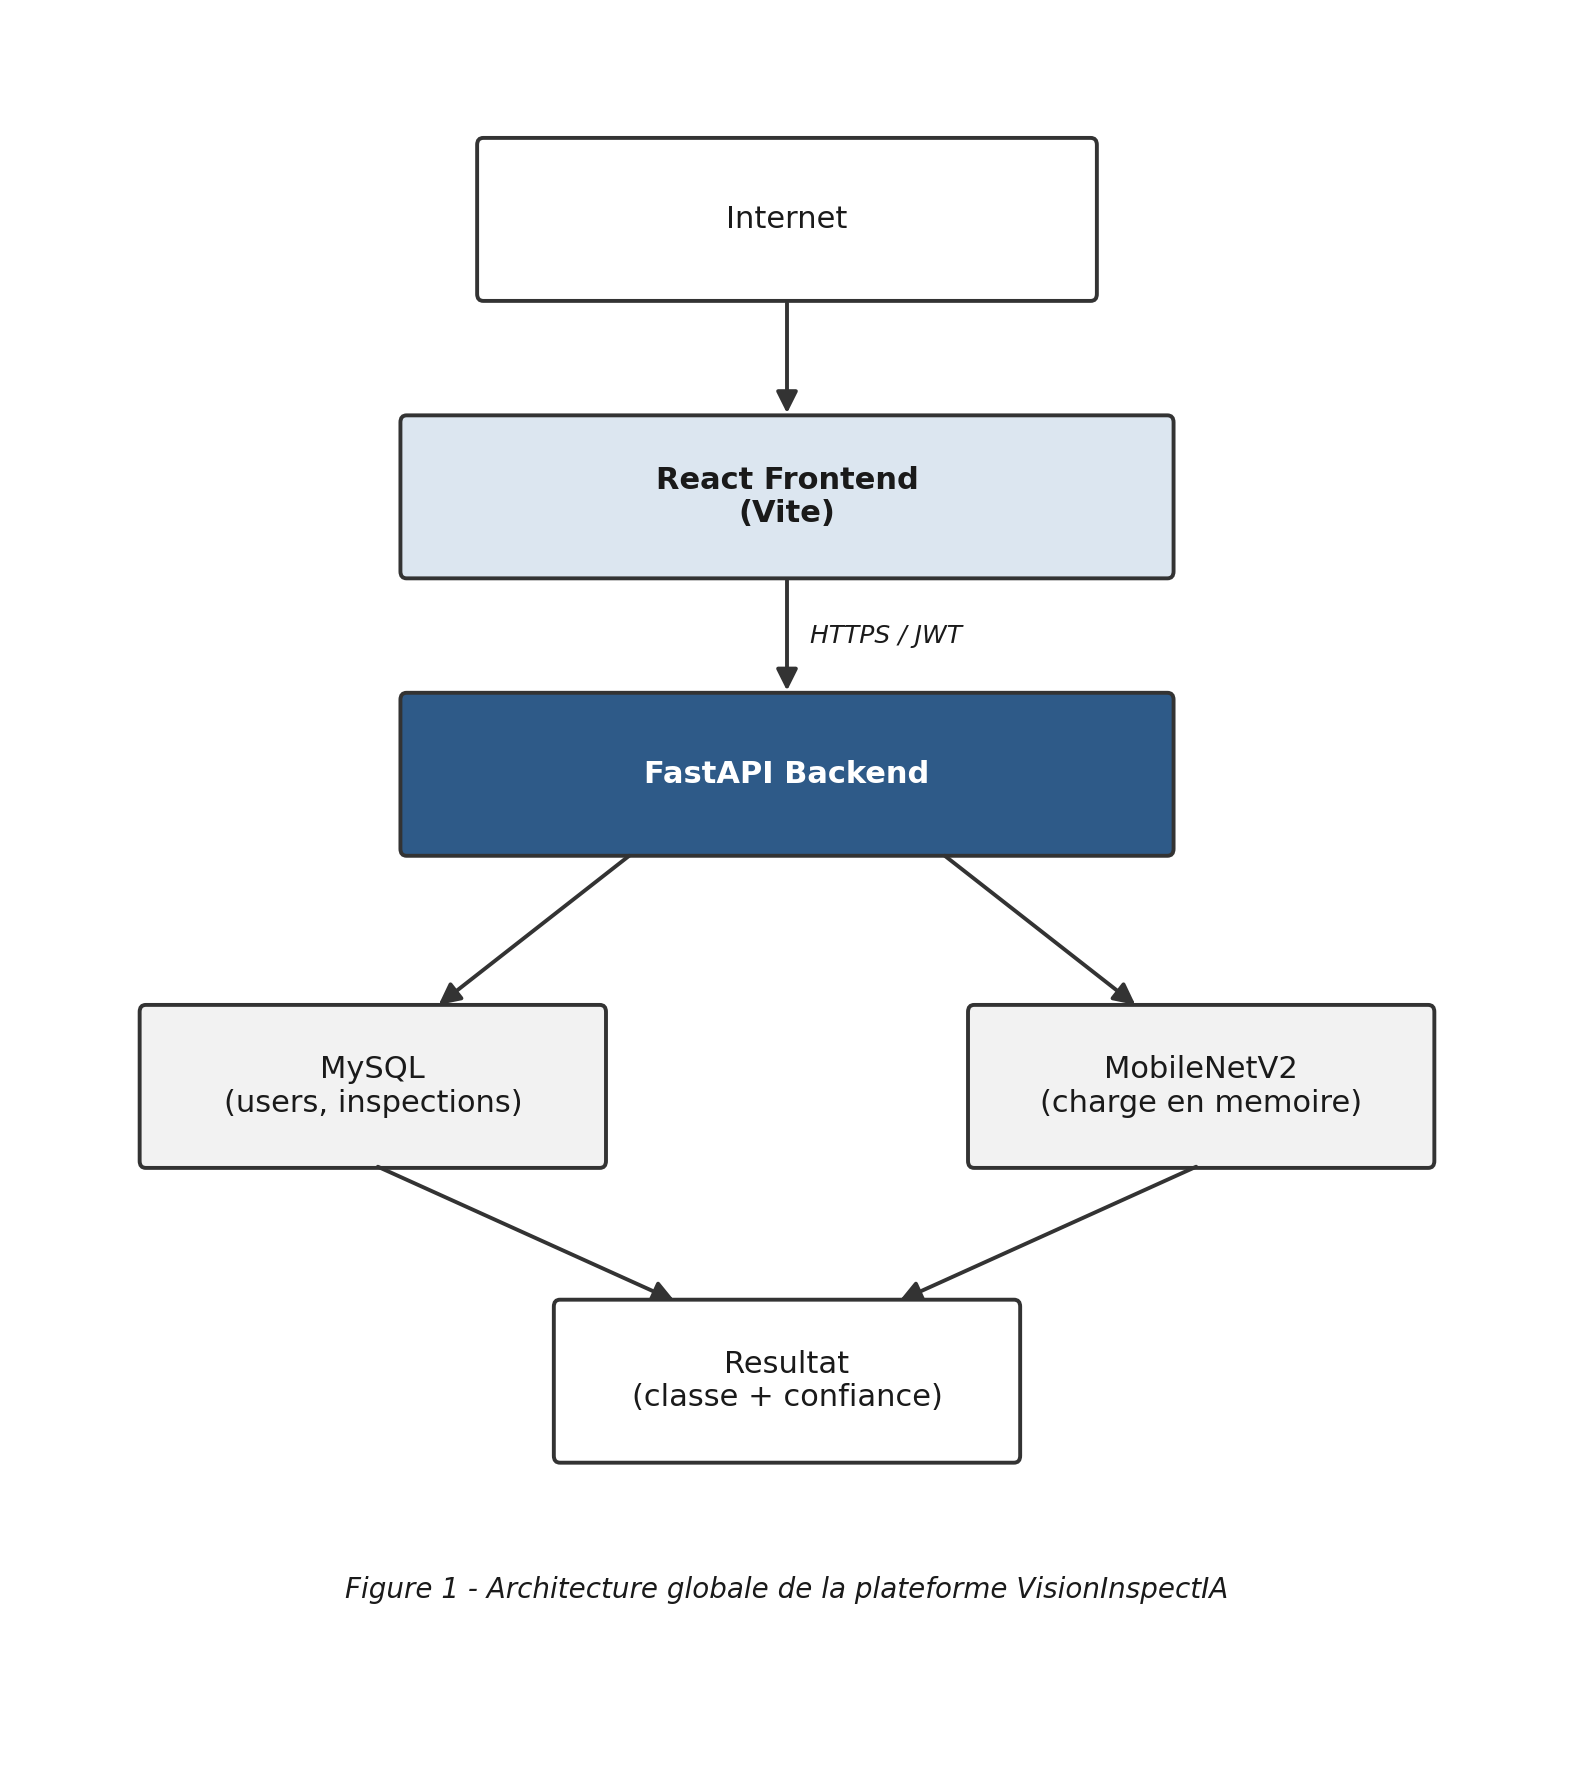
\includegraphics[width=0.65\textwidth]{figure_01_architecture_globale.png}
\caption{Rappel~: architecture globale de la plateforme VisionInspectIA.}
\end{figure}

\chapter{Endpoints de l'API}
\label{annex:api}

Voir \Cref{tab:endpoints} (\Cref{ch:backend}) pour la liste compl\`ete des endpoints r\'eellement expos\'es par l'API REST (source~: \texttt{backend/app/api/v1/router.py}).

\chapter{Base de donn\'ees}
\label{annex:database}

Voir \Cref{ch:database}, \Cref{tab:table-users}, \Cref{tab:table-inspections} et \Cref{fig:erd}.

\chapter{R\'esultats IA}
\label{annex:results}

Voir \Cref{tab:benchmark} et \Cref{tab:classification-report} (\Cref{ch:modelisation}).

\section*{Correspondance avec le cahier des charges}

\begin{table}[H]
\centering
\small
\caption{Correspondance exigences du cahier des charges / r\'ealisation}
\label{tab:cahier-des-charges}
\begin{tabularx}{\textwidth}{lXl}
\toprule
Exigence & R\'ealisation & Preuve \\
\midrule
Dataset & MVTec AD, cat\'egorie bottle & \Cref{ch:dataset} \\
4~mod\`eles & CNN / MobileNetV2 / EfficientNetB0 / ResNet50 & \Cref{ch:modelisation} \\
Accuracy & Oui & \Cref{tab:benchmark} \\
Precision & Oui & \Cref{tab:benchmark} \\
Recall & Oui & \Cref{tab:benchmark} \\
F1-score & Oui & \Cref{tab:benchmark} \\
Matrice de confusion & Oui & \Cref{fig:confusion-matrix} \\
Courbe ROC & \textbf{Non disponible} --- aucun fichier trouv\'e dans \texttt{ai/results/} & \Cref{ch:modelisation} \\
React & Oui & \Cref{ch:frontend} \\
FastAPI & Oui & \Cref{ch:backend} \\
MySQL & Oui & \Cref{ch:database} \\
Authentification & Oui (JWT) & \Cref{ch:backend} \\
Upload & Oui & \Cref{ch:ia-prediction} \\
Historique & Oui & \Cref{ch:frontend} \\
PDF & Oui & \Cref{ch:backend}, \Cref{ch:frontend} \\
Dashboard & Oui & \Cref{ch:frontend} \\
D\'eploiement cloud & Railway & \Cref{ch:deploiement} \\
Format mod\`ele \texttt{.h5}/\texttt{.pt} & \textbf{Non} --- format \texttt{.keras} utilis\'e \`a la place & \Cref{ch:modelisation} \\
Pr\'esentation (PPT) & [\`A COMPL\'ETER] --- non produit dans le cadre de ce rapport LaTeX & --- \\
Vid\'eo de d\'emonstration & [\`A COMPL\'ETER] --- non enregistr\'ee \`a ce jour & --- \\
\bottomrule
\end{tabularx}
\end{table}

\begin{noteflag}{Important}
La courbe ROC n'est pas pr\'esent\'ee comme existante~: aucun fichier correspondant n'a \'et\'e retrouv\'e dans \texttt{ai/results/}, et aucune courbe n'a \'et\'e invent\'ee pour combler cette absence.
\end{noteflag}

\chapter{Captures de la plateforme}
\label{annex:captures}

Aucune capture d'\'ecran n'a \'et\'e produite dans le cadre de la r\'edaction de ce rapport (environnement de d\'eveloppement sans navigateur graphique). Les captures suivantes restent \`a r\'ealiser avant la finalisation du rapport~:

\begin{enumerate}
  \item [CAPTURE \`A AJOUTER] Login
  \item [CAPTURE \`A AJOUTER] Register
  \item [CAPTURE \`A AJOUTER] Dashboard
  \item [CAPTURE \`A AJOUTER] Prediction (interface d'upload)
  \item [CAPTURE \`A AJOUTER] R\'esultat de pr\'ediction (classe, confiance, temps d'inf\'erence)
  \item [CAPTURE \`A AJOUTER] History
  \item [CAPTURE \`A AJOUTER] Inspection details (modal)
  \item [CAPTURE \`A AJOUTER] PDF g\'en\'er\'e
  \item [CAPTURE \`A AJOUTER] Export CSV
  \item [CAPTURE \`A AJOUTER] Profile
  \item [CAPTURE \`A AJOUTER] Dark mode
  \item Swagger --- r\'ealisable imm\'ediatement \`a l'URL \url{https://visioninspectia-production.up.railway.app/docs}
  \item [CAPTURE \`A AJOUTER] Railway --- service frontend
  \item [CAPTURE \`A AJOUTER] Railway --- service backend
\end{enumerate}

\chapter{D\'eploiement}
\label{annex:deploiement}

Voir \Cref{ch:deploiement}, URLs list\'ees en \Cref{sec:urls}, probl\`emes et solutions en \Cref{sec:problemes-deploiement}.


\end{document}
